\chapter{Análisis semántico: chequeo de sentencias}
\label{cap:semantico-sentencias}
\begingroup
\setlength{\emergencystretch}{4em}

Esta etapa construye los árboles sintácticos abstractos de los cuerpos
de métodos, constructores y del bloque \texttt{start}. A partir de la
tabla de símbolos consolidada, comprueba las expresiones, asignaciones,
llamadas, condiciones, recorridos y retornos.

\section{Diseño y ejecución de la etapa}
\label{sec:diseno-sentencias}

\begin{description}[style=nextline]
  \item[Reconocimiento y construcción]
  \lexcode{SemanticAnalyzer} crea los nodos al reconocer las producciones
  de la gramática. Las declaraciones se registran en la tabla; los
  cuerpos se guardan como árboles de sentencias y expresiones.
  \item[Chequeo]
  \lexcode{TypeVisitor} implementa \lexcode{Visitor<Type>}. Cada nodo
  selecciona la sobrecarga correspondiente mediante \lexcode{accept()}.
  Las expresiones devuelven su tipo; las sentencias comprueban sus hijos
  y actualizan la información de retorno cuando corresponde.
  \item[Exportación]
  \lexcode{AstJsonVisitor} implementa \lexcode{Visitor<Object>} y
  construye la representación que serializa \lexcode{JsonWriter}.
  El archivo de tabla se obtiene de \lexcode{SymbolTable.toJson()}.
\end{description}


La compilación y ejecución desde la raíz del proyecto son:
\begin{verbatim}
mvn -Petapa4 -DskipTests package
java -jar target/etapa4.jar <ARCH_FUENTE>.s
\end{verbatim}
Si tanto el chequeo de declaraciones como el de sentencias terminan correctamente, se muestra:
\begin{verbatim}
CORRECTO: SEMANTICO - SENTENCIAS
\end{verbatim}
Se escriben \texttt{<ARCH\_FUENTE>.ts.json} y
\texttt{<ARCH\_FUENTE>.ast.json} junto al archivo fuente. El nombre
base se conserva y la escritura reemplaza los resultados anteriores.

\section{Esquema de traducción}
\label{sec:edt-sentencias}

% Transcripción del EDT de sentencias proporcionado por el autor.
% https://docs.google.com/document/d/1fLvQLmMxuIsQLP6FdxHd5cRqd1_4q0jBzG1xYV_XgVE/edit
% Se conservan el texto, el orden y los tramos resaltados del documento fuente.
\begingroup
\definecolor{edtAstVerde}{RGB}{213,242,220}
\newcommand{\astaccion}[1]{{\setlength{\fboxsep}{0pt}\colorbox{edtAstVerde}{\strut #1}}}
\newcommand{\astlinea}[1]{\hangindent=1.6em\hangafter=1\noindent#1\par}
\begin{tcolorbox}[enhanced jigsaw,breakable,sharp corners,colback=white,colframe=gray,boxrule=0.4pt,boxsep=0pt,left=4pt,right=4pt,top=4pt,bottom=4pt]
\par\addvspace{0.6em}
\noindent\begin{minipage}{\linewidth}
\ttfamily\small\raggedright
\setlength{\parindent}{0pt}
\setlength{\parskip}{0pt}
\astlinea{\ensuremath{\langle}program\ensuremath{\rangle} ::= \astaccion{\{} \astaccion{AST} \astaccion{=} \astaccion{new} \astaccion{AST}\astaccion{(}\allowbreak{}\astaccion{)}\allowbreak{} \astaccion{\}} \ensuremath{\langle}Lista-{}Definiciones\ensuremath{\rangle} \ensuremath{\langle}Start\ensuremath{\rangle} \astaccion{\{AST}\astaccion{.}\allowbreak{}\astaccion{setSymbolTable}\astaccion{(}\allowbreak{}\astaccion{this}\astaccion{)}\allowbreak{}\astaccion{,}\allowbreak{} \astaccion{AST}\astaccion{.}\allowbreak{}\astaccion{consolidate}\astaccion{(}\allowbreak{}\astaccion{)}\allowbreak{} \astaccion{\}}}
\end{minipage}\par
\par\addvspace{0.6em}
\noindent\begin{minipage}{\linewidth}
\ttfamily\small\raggedright
\setlength{\parindent}{0pt}
\setlength{\parskip}{0pt}
\astlinea{\ensuremath{\langle}Start\ensuremath{\rangle} ::= start \ensuremath{\langle}Bloque-{}Método\ensuremath{\rangle}}
\end{minipage}\par
\par\addvspace{0.6em}
\noindent\begin{minipage}{\linewidth}
\ttfamily\small\raggedright
\setlength{\parindent}{0pt}
\setlength{\parskip}{0pt}
\astlinea{\ensuremath{\langle}Lista-{}Definiciones\ensuremath{\rangle} ::= \ensuremath{\langle}class\ensuremath{\rangle} \ensuremath{\langle}Lista-{}Definiciones\ensuremath{\rangle}}
\end{minipage}\par
\noindent\begin{minipage}{\linewidth}
\ttfamily\small\raggedright
\setlength{\parindent}{0pt}
\setlength{\parskip}{0pt}
\astlinea{\hspace*{1.6em}\textbar{} \ensuremath{\langle}Impl\ensuremath{\rangle} \ensuremath{\langle}Lista-{}Definiciones\ensuremath{\rangle}}
\end{minipage}\par
\noindent\begin{minipage}{\linewidth}
\ttfamily\small\raggedright
\setlength{\parindent}{0pt}
\setlength{\parskip}{0pt}
\astlinea{\hspace*{1.6em}\textbar{} \ensuremath{\lambda}}
\end{minipage}\par
\par\addvspace{0.6em}
\noindent\begin{minipage}{\linewidth}
\ttfamily\small\raggedright
\setlength{\parindent}{0pt}
\setlength{\parskip}{0pt}
\astlinea{\ensuremath{\langle}class\ensuremath{\rangle} ::= class idclass \ensuremath{\langle}classF\ensuremath{\rangle}}
\end{minipage}\par
\par\addvspace{0.6em}
\noindent\begin{minipage}{\linewidth}
\ttfamily\small\raggedright
\setlength{\parindent}{0pt}
\setlength{\parskip}{0pt}
\astlinea{\ensuremath{\langle}classF\ensuremath{\rangle} ::= \{ \ensuremath{\langle}AtributoK\ensuremath{\rangle} \}}
\end{minipage}\par
\noindent\begin{minipage}{\linewidth}
\ttfamily\small\raggedright
\setlength{\parindent}{0pt}
\setlength{\parskip}{0pt}
\astlinea{\hspace*{1.6em}\textbar{} \ensuremath{\langle}Herencia\ensuremath{\rangle} \{ \ensuremath{\langle}AtributoK\ensuremath{\rangle} \}}
\end{minipage}\par
\par\addvspace{0.6em}
\noindent\begin{minipage}{\linewidth}
\ttfamily\small\raggedright
\setlength{\parindent}{0pt}
\setlength{\parskip}{0pt}
\astlinea{\ensuremath{\langle}AtributoK\ensuremath{\rangle} ::= \ensuremath{\langle}Atributo\ensuremath{\rangle} \ensuremath{\langle}AtributoK\ensuremath{\rangle}}
\end{minipage}\par
\noindent\begin{minipage}{\linewidth}
\ttfamily\small\raggedright
\setlength{\parindent}{0pt}
\setlength{\parskip}{0pt}
\astlinea{\hspace*{1.6em}\textbar{} \ensuremath{\lambda}}
\end{minipage}\par
\par\addvspace{0.6em}
\noindent\begin{minipage}{\linewidth}
\ttfamily\small\raggedright
\setlength{\parindent}{0pt}
\setlength{\parskip}{0pt}
\astlinea{\ensuremath{\langle}Impl\ensuremath{\rangle} ::= impl idclass \{ \ensuremath{\langle}MiembroK\ensuremath{\rangle} \}}
\end{minipage}\par
\par\addvspace{0.6em}
\noindent\begin{minipage}{\linewidth}
\ttfamily\small\raggedright
\setlength{\parindent}{0pt}
\setlength{\parskip}{0pt}
\astlinea{\ensuremath{\langle}Herencia\ensuremath{\rangle} ::= : \ensuremath{\langle}Tipo\ensuremath{\rangle}}
\end{minipage}\par
\par\addvspace{0.6em}
\noindent\begin{minipage}{\linewidth}
\ttfamily\small\raggedright
\setlength{\parindent}{0pt}
\setlength{\parskip}{0pt}
\astlinea{\ensuremath{\langle}MiembroK\ensuremath{\rangle} ::= \ensuremath{\langle}Miembro\ensuremath{\rangle} \ensuremath{\langle}MiembroK\ensuremath{\rangle}}
\end{minipage}\par
\noindent\begin{minipage}{\linewidth}
\ttfamily\small\raggedright
\setlength{\parindent}{0pt}
\setlength{\parskip}{0pt}
\astlinea{\hspace*{1.6em}\textbar{} \ensuremath{\lambda}}
\end{minipage}\par
\par\addvspace{0.6em}
\noindent\begin{minipage}{\linewidth}
\ttfamily\small\raggedright
\setlength{\parindent}{0pt}
\setlength{\parskip}{0pt}
\astlinea{\ensuremath{\langle}Miembro\ensuremath{\rangle} ::= \ensuremath{\langle}Método\ensuremath{\rangle}}
\end{minipage}\par
\noindent\begin{minipage}{\linewidth}
\ttfamily\small\raggedright
\setlength{\parindent}{0pt}
\setlength{\parskip}{0pt}
\astlinea{\hspace*{1.6em}\textbar{} \ensuremath{\langle}Constructor\ensuremath{\rangle}}
\end{minipage}\par
\par\addvspace{0.6em}
\noindent\begin{minipage}{\linewidth}
\ttfamily\small\raggedright
\setlength{\parindent}{0pt}
\setlength{\parskip}{0pt}
\astlinea{\ensuremath{\langle}Constructor\ensuremath{\rangle} ::= . \ensuremath{\langle}Argumentos-{}Formales\ensuremath{\rangle} \ensuremath{\langle}Bloque-{}Método\ensuremath{\rangle}}
\end{minipage}\par
\par\addvspace{0.6em}
\noindent\begin{minipage}{\linewidth}
\ttfamily\small\raggedright
\setlength{\parindent}{0pt}
\setlength{\parskip}{0pt}
\astlinea{\ensuremath{\langle}Atributo\ensuremath{\rangle} ::= \ensuremath{\langle}Tipo\ensuremath{\rangle} \ensuremath{\langle}Lista-{}Declaración-{}Variables\ensuremath{\rangle} ;}
\end{minipage}\par
\noindent\begin{minipage}{\linewidth}
\ttfamily\small\raggedright
\setlength{\parindent}{0pt}
\setlength{\parskip}{0pt}
\astlinea{\hspace*{1.6em}\textbar{} pub \ensuremath{\langle}Tipo\ensuremath{\rangle} \ensuremath{\langle}Lista-{}Declaración-{}Variables\ensuremath{\rangle} ;}
\end{minipage}\par
\par\addvspace{0.6em}
\noindent\begin{minipage}{\linewidth}
\ttfamily\small\raggedright
\setlength{\parindent}{0pt}
\setlength{\parskip}{0pt}
\astlinea{\ensuremath{\langle}Método\ensuremath{\rangle} ::= fn \ensuremath{\langle}MétodoF\ensuremath{\rangle}}
\end{minipage}\par
\noindent\begin{minipage}{\linewidth}
\ttfamily\small\raggedright
\setlength{\parindent}{0pt}
\setlength{\parskip}{0pt}
\astlinea{\hspace*{1.6em}\textbar{} st fn \ensuremath{\langle}MétodoF\ensuremath{\rangle}}
\end{minipage}\par
\par\addvspace{0.6em}
\noindent\begin{minipage}{\linewidth}
\ttfamily\small\raggedright
\setlength{\parindent}{0pt}
\setlength{\parskip}{0pt}
\astlinea{\ensuremath{\langle}MétodoF\ensuremath{\rangle} ::= idMetAt \ensuremath{\langle}Argumentos-{}Formales\ensuremath{\rangle} \ensuremath{\langle}Bloque-{}Método\ensuremath{\rangle}}
\end{minipage}\par
\noindent\begin{minipage}{\linewidth}
\ttfamily\small\raggedright
\setlength{\parindent}{0pt}
\setlength{\parskip}{0pt}
\astlinea{\hspace*{1.6em}\textbar{} \ensuremath{\langle}Tipo-{}Método\ensuremath{\rangle} idMetAt \ensuremath{\langle}Argumentos-{}Formales\ensuremath{\rangle} \ensuremath{\langle}Bloque-{}Método\ensuremath{\rangle}}
\end{minipage}\par
\par\addvspace{0.6em}
\noindent\begin{minipage}{\linewidth}
\ttfamily\small\raggedright
\setlength{\parindent}{0pt}
\setlength{\parskip}{0pt}
\astlinea{\ensuremath{\langle}Bloque-{}Método\ensuremath{\rangle} ::= \{ \ensuremath{\langle}Decl-{}Var-{}LocalesK\ensuremath{\rangle} \astaccion{\{sentenceNodeList} \astaccion{=} \astaccion{new} \astaccion{List}\astaccion{(}\allowbreak{}\astaccion{)}\allowbreak{}\astaccion{,}\allowbreak{} \astaccion{sentenciaK}\astaccion{.}\allowbreak{}\astaccion{setSentenceNodes}\astaccion{(}\allowbreak{} \astaccion{sentenceNodeList}\astaccion{)}\allowbreak{}\astaccion{\}} \ensuremath{\langle}SentenciaK\ensuremath{\rangle} \} \astaccion{\{currentBlockNode} \astaccion{=} \astaccion{newBlackNode}\astaccion{(}\allowbreak{}\astaccion{sentenciaK}\astaccion{.}\allowbreak{}\astaccion{getSentenceNodes}\astaccion{(}\allowbreak{}\astaccion{)}\allowbreak{}\astaccion{,}\allowbreak{} \astaccion{TS}\astaccion{.}\allowbreak{}\astaccion{getCurrentClass}\astaccion{(}\allowbreak{}\astaccion{)}\allowbreak{}\astaccion{,}\allowbreak{} \astaccion{TS}\astaccion{.}\allowbreak{}\astaccion{getCurrentMethod}\astaccion{(}\allowbreak{}\astaccion{)}\allowbreak{}\astaccion{)}\allowbreak{} \astaccion{iif} \astaccion{currentMethod} \astaccion{==} \astaccion{start} \astaccion{then} \astaccion{AST}\astaccion{.}\allowbreak{}\astaccion{setStartBlockNode}\astaccion{(}\allowbreak{}\astaccion{currentBlockNode}\astaccion{)}\allowbreak{} \astaccion{else} \astaccion{AST}\astaccion{.}\allowbreak{}\astaccion{addBlockNode}\astaccion{(}\allowbreak{}\astaccion{currentBlockNode}\astaccion{)}\allowbreak{}\astaccion{\}}}
\end{minipage}\par
\par\addvspace{0.6em}
\noindent\begin{minipage}{\linewidth}
\ttfamily\small\raggedright
\setlength{\parindent}{0pt}
\setlength{\parskip}{0pt}
\astlinea{\ensuremath{\langle}Decl-{}Var-{}LocalesK\ensuremath{\rangle} ::= \ensuremath{\langle}Decl-{}Var-{}Locales\ensuremath{\rangle} \ensuremath{\langle}Decl-{}Var-{}LocalesK\ensuremath{\rangle}}
\end{minipage}\par
\noindent\begin{minipage}{\linewidth}
\ttfamily\small\raggedright
\setlength{\parindent}{0pt}
\setlength{\parskip}{0pt}
\astlinea{\hspace*{1.6em}\textbar{} \ensuremath{\lambda}}
\end{minipage}\par
\par\addvspace{0.6em}
\noindent\begin{minipage}{\linewidth}
\ttfamily\small\raggedright
\setlength{\parindent}{0pt}
\setlength{\parskip}{0pt}
\astlinea{\ensuremath{\langle}Decl-{}Var-{}Locales\ensuremath{\rangle} ::= \ensuremath{\langle}Tipo\ensuremath{\rangle} \ensuremath{\langle}Lista-{}Declaración-{}Variables\ensuremath{\rangle} ;}
\end{minipage}\par
\par\addvspace{0.6em}
\noindent\begin{minipage}{\linewidth}
\ttfamily\small\raggedright
\setlength{\parindent}{0pt}
\setlength{\parskip}{0pt}
\astlinea{\ensuremath{\langle}Lista-{}Declaración-{}Variables\ensuremath{\rangle} ::= idMetAt \ensuremath{\langle}Lista-{}Declaración-{}VariablesF\ensuremath{\rangle}}
\end{minipage}\par
\par\addvspace{0.6em}
\noindent\begin{minipage}{\linewidth}
\ttfamily\small\raggedright
\setlength{\parindent}{0pt}
\setlength{\parskip}{0pt}
\astlinea{\ensuremath{\langle}Lista-{}Declaración-{}VariablesF\ensuremath{\rangle} ::= , \ensuremath{\langle}Lista-{}Declaración-{}Variables\ensuremath{\rangle}}
\end{minipage}\par
\noindent\begin{minipage}{\linewidth}
\ttfamily\small\raggedright
\setlength{\parindent}{0pt}
\setlength{\parskip}{0pt}
\astlinea{\hspace*{1.6em}\textbar{} \ensuremath{\lambda}}
\end{minipage}\par
\par\addvspace{0.6em}
\noindent\begin{minipage}{\linewidth}
\ttfamily\small\raggedright
\setlength{\parindent}{0pt}
\setlength{\parskip}{0pt}
\astlinea{\ensuremath{\langle}Argumentos-{}Formales\ensuremath{\rangle} ::= ( \ensuremath{\langle}Argumentos-{}FormalesF\ensuremath{\rangle}}
\end{minipage}\par
\par\addvspace{0.6em}
\noindent\begin{minipage}{\linewidth}
\ttfamily\small\raggedright
\setlength{\parindent}{0pt}
\setlength{\parskip}{0pt}
\astlinea{\ensuremath{\langle}Argumentos-{}FormalesF\ensuremath{\rangle} ::= )}
\end{minipage}\par
\noindent\begin{minipage}{\linewidth}
\ttfamily\small\raggedright
\setlength{\parindent}{0pt}
\setlength{\parskip}{0pt}
\astlinea{\hspace*{1.6em}\textbar{} \ensuremath{\langle}Lista-{}Argumentos-{}Formales\ensuremath{\rangle} )}
\end{minipage}\par
\par\addvspace{0.6em}
\noindent\begin{minipage}{\linewidth}
\ttfamily\small\raggedright
\setlength{\parindent}{0pt}
\setlength{\parskip}{0pt}
\astlinea{\ensuremath{\langle}Lista-{}Argumentos-{}Formales\ensuremath{\rangle} ::= \ensuremath{\langle}Argumento-{}Formal\ensuremath{\rangle} \ensuremath{\langle}Lista-{}Argumentos-{}FormalesF\ensuremath{\rangle}}
\end{minipage}\par
\par\addvspace{0.6em}
\noindent\begin{minipage}{\linewidth}
\ttfamily\small\raggedright
\setlength{\parindent}{0pt}
\setlength{\parskip}{0pt}
\astlinea{\ensuremath{\langle}Lista-{}Argumentos-{}FormalesF\ensuremath{\rangle} ::= , \ensuremath{\langle}Lista-{}Argumentos-{}Formales\ensuremath{\rangle}}
\end{minipage}\par
\noindent\begin{minipage}{\linewidth}
\ttfamily\small\raggedright
\setlength{\parindent}{0pt}
\setlength{\parskip}{0pt}
\astlinea{\hspace*{1.6em}\textbar{} \ensuremath{\lambda}}
\end{minipage}\par
\par\addvspace{0.6em}
\noindent\begin{minipage}{\linewidth}
\ttfamily\small\raggedright
\setlength{\parindent}{0pt}
\setlength{\parskip}{0pt}
\astlinea{\ensuremath{\langle}Argumento-{}Formal\ensuremath{\rangle} ::= \ensuremath{\langle}Tipo\ensuremath{\rangle} idMetAt}
\end{minipage}\par
\par\addvspace{0.6em}
\noindent\begin{minipage}{\linewidth}
\ttfamily\small\raggedright
\setlength{\parindent}{0pt}
\setlength{\parskip}{0pt}
\astlinea{\ensuremath{\langle}Tipo-{}Método\ensuremath{\rangle} ::= \ensuremath{\langle}Tipo\ensuremath{\rangle}}
\end{minipage}\par
\noindent\begin{minipage}{\linewidth}
\ttfamily\small\raggedright
\setlength{\parindent}{0pt}
\setlength{\parskip}{0pt}
\astlinea{\hspace*{1.6em}\textbar{} void}
\end{minipage}\par
\par\addvspace{0.6em}
\noindent\begin{minipage}{\linewidth}
\ttfamily\small\raggedright
\setlength{\parindent}{0pt}
\setlength{\parskip}{0pt}
\astlinea{\ensuremath{\langle}Tipo\ensuremath{\rangle} ::= \ensuremath{\langle}Tipo-{}Primitivo\ensuremath{\rangle}}
\end{minipage}\par
\noindent\begin{minipage}{\linewidth}
\ttfamily\small\raggedright
\setlength{\parindent}{0pt}
\setlength{\parskip}{0pt}
\astlinea{\hspace*{1.6em}\textbar{} \ensuremath{\langle}Tipo-{}Referencia\ensuremath{\rangle}}
\end{minipage}\par
\noindent\begin{minipage}{\linewidth}
\ttfamily\small\raggedright
\setlength{\parindent}{0pt}
\setlength{\parskip}{0pt}
\astlinea{\hspace*{1.6em}\textbar{} \ensuremath{\langle}Tipo-{}Arreglo\ensuremath{\rangle}}
\end{minipage}\par
\par\addvspace{0.6em}
\noindent\begin{minipage}{\linewidth}
\ttfamily\small\raggedright
\setlength{\parindent}{0pt}
\setlength{\parskip}{0pt}
\astlinea{\ensuremath{\langle}Tipo-{}Primitivo\ensuremath{\rangle} ::= Str}
\end{minipage}\par
\noindent\begin{minipage}{\linewidth}
\ttfamily\small\raggedright
\setlength{\parindent}{0pt}
\setlength{\parskip}{0pt}
\astlinea{\hspace*{1.6em}\textbar{} Bool}
\end{minipage}\par
\noindent\begin{minipage}{\linewidth}
\ttfamily\small\raggedright
\setlength{\parindent}{0pt}
\setlength{\parskip}{0pt}
\astlinea{\hspace*{1.6em}\textbar{} Int}
\end{minipage}\par
\par\addvspace{0.6em}
\noindent\begin{minipage}{\linewidth}
\ttfamily\small\raggedright
\setlength{\parindent}{0pt}
\setlength{\parskip}{0pt}
\astlinea{\ensuremath{\langle}Tipo-{}Referencia\ensuremath{\rangle} ::= idclass}
\end{minipage}\par
\par\addvspace{0.6em}
\noindent\begin{minipage}{\linewidth}
\ttfamily\small\raggedright
\setlength{\parindent}{0pt}
\setlength{\parskip}{0pt}
\astlinea{\ensuremath{\langle}Tipo-{}Arreglo\ensuremath{\rangle} ::= Array \ensuremath{\langle}Tipo-{}Primitivo\ensuremath{\rangle}}
\end{minipage}\par
\par\addvspace{0.6em}
\noindent\begin{minipage}{\linewidth}
\ttfamily\small\raggedright
\setlength{\parindent}{0pt}
\setlength{\parskip}{0pt}
\astlinea{\ensuremath{\langle}SentenciaK1\ensuremath{\rangle} ::= \ensuremath{\langle}Sentencia\ensuremath{\rangle} \astaccion{\{SentenciaK1}\astaccion{.}\allowbreak{}\astaccion{getSentenceNodes}\astaccion{(}\allowbreak{}\astaccion{)}\allowbreak{}\astaccion{.}\allowbreak{}\astaccion{add}\astaccion{(}\allowbreak{}\astaccion{Sentencia}\astaccion{.}\allowbreak{}\astaccion{getSentenceNode}\astaccion{(}\allowbreak{}\astaccion{)}\allowbreak{}\astaccion{)}\allowbreak{}\astaccion{,}\allowbreak{} \astaccion{SentenciaK2}\astaccion{.}\allowbreak{}\astaccion{setSentenceNodes}\astaccion{(}\allowbreak{}\astaccion{SentenciaK1}\astaccion{.}\allowbreak{}\astaccion{getSentenceNodes}\astaccion{(}\allowbreak{}\astaccion{)}\allowbreak{}\astaccion{\}}  \ensuremath{\langle}SentenciaK2\ensuremath{\rangle} \astaccion{\{SentenciaK1}\astaccion{.}\allowbreak{}\astaccion{setSentenceNodes}\astaccion{(}\allowbreak{}\astaccion{SentenciaK2}\astaccion{.}\allowbreak{}\astaccion{getSentenceNodes}\astaccion{(}\allowbreak{}\astaccion{)}\allowbreak{}\astaccion{)}\allowbreak{}\astaccion{\}}}
\end{minipage}\par
\noindent\begin{minipage}{\linewidth}
\ttfamily\small\raggedright
\setlength{\parindent}{0pt}
\setlength{\parskip}{0pt}
\astlinea{\hspace*{1.6em}\textbar{} \ensuremath{\lambda}}
\end{minipage}\par
\par\addvspace{0.6em}
\noindent\begin{minipage}{\linewidth}
\ttfamily\small\raggedright
\setlength{\parindent}{0pt}
\setlength{\parskip}{0pt}
\astlinea{\ensuremath{\langle}Sentencia\ensuremath{\rangle} ::= \astaccion{\{sentenceNode} \astaccion{=} \astaccion{null\}} ; \astaccion{\{Sentencia}\astaccion{.}\allowbreak{}\astaccion{setSentenceNode}\astaccion{(}\allowbreak{}\astaccion{sentenceNode}\astaccion{)}\allowbreak{}\astaccion{\}}}
\end{minipage}\par
\noindent\begin{minipage}{\linewidth}
\ttfamily\small\raggedright
\setlength{\parindent}{0pt}
\setlength{\parskip}{0pt}
\astlinea{\hspace*{1.6em}\textbar{} \astaccion{\{sentenceNode} \astaccion{=} \astaccion{null\}} \ensuremath{\langle}Asignación\ensuremath{\rangle} \astaccion{\{} \astaccion{sentenceNode} \astaccion{=} \astaccion{Asignación}\astaccion{.}\allowbreak{}\astaccion{getSentenceNode}\astaccion{(}\allowbreak{}\astaccion{)}\allowbreak{}\astaccion{\}} ; \astaccion{\{Sentencia}\astaccion{.}\allowbreak{}\astaccion{setSentenceNode}\astaccion{(}\allowbreak{}\astaccion{sentenceNode}\astaccion{)}\allowbreak{}\astaccion{\}}}
\end{minipage}\par
\noindent\begin{minipage}{\linewidth}
\ttfamily\small\raggedright
\setlength{\parindent}{0pt}
\setlength{\parskip}{0pt}
\astlinea{\hspace*{1.6em}\textbar{} \astaccion{\{sentenceNode} \astaccion{=} \astaccion{null\}} \ensuremath{\langle}Sentencia-{}Simple\ensuremath{\rangle} \astaccion{\{} \astaccion{sentenceNode} \astaccion{=} \astaccion{Sentencia-{}Simple}\astaccion{.}\allowbreak{}\astaccion{getSentenceNode}\astaccion{(}\allowbreak{}\astaccion{)}\allowbreak{} \astaccion{\}} ; \astaccion{\{Sentencia}\astaccion{.}\allowbreak{}\astaccion{setSentenceNode}\astaccion{(}\allowbreak{}\astaccion{sentenceNode}\astaccion{)}\allowbreak{}\astaccion{\}}}
\end{minipage}\par
\noindent\begin{minipage}{\linewidth}
\ttfamily\small\raggedright
\setlength{\parindent}{0pt}
\setlength{\parskip}{0pt}
\astlinea{\hspace*{1.6em}\textbar{} \astaccion{\{sentenceNode} \astaccion{=} \astaccion{null\}} while ( \ensuremath{\langle}Expresión\ensuremath{\rangle} \astaccion{\{expressionNode} \astaccion{=} \astaccion{Expresion}\astaccion{.}\allowbreak{}\astaccion{getExpressionNode}\astaccion{(}\allowbreak{}\astaccion{)}\allowbreak{}\astaccion{\}} ) \ensuremath{\langle}Sentencia\ensuremath{\rangle} \astaccion{\{} \astaccion{sentenceNode} \astaccion{=} \astaccion{new} \astaccion{WhileNode}\astaccion{(}\allowbreak{}\astaccion{tokenWhile}\astaccion{,}\allowbreak{} \astaccion{expressionNode}\astaccion{,}\allowbreak{} \astaccion{sentencia}\astaccion{.}\allowbreak{}\astaccion{getSentenceNode}\astaccion{(}\allowbreak{}\astaccion{)}\allowbreak{}\astaccion{)}\allowbreak{}\astaccion{,}\allowbreak{} \astaccion{Sentencia}\astaccion{.}\allowbreak{}\astaccion{setSentenceNode}\astaccion{(}\allowbreak{}\astaccion{sentenceNode}\astaccion{)}\allowbreak{}\astaccion{\}}}
\end{minipage}\par
\noindent\begin{minipage}{\linewidth}
\ttfamily\small\raggedright
\setlength{\parindent}{0pt}
\setlength{\parskip}{0pt}
\astlinea{\hspace*{1.6em}\textbar{} \astaccion{\{sentenceNode} \astaccion{=} \astaccion{null\}} for ( \ensuremath{\langle}Tipo-{}Primitivo\ensuremath{\rangle} idMetAt1 \astaccion{\{variableNode1} \astaccion{=} \astaccion{new} \astaccion{VariableNode}\astaccion{(}\allowbreak{}\astaccion{idMetAt1}\astaccion{.}\allowbreak{}\astaccion{token}\astaccion{,}\allowbreak{} \astaccion{null}\astaccion{,}\allowbreak{} \astaccion{TS}\astaccion{.}\allowbreak{}\astaccion{getCurrentClass}\astaccion{(}\allowbreak{}\astaccion{)}\allowbreak{}\astaccion{,}\allowbreak{} \astaccion{TS}\astaccion{.}\allowbreak{}\astaccion{getCurrentMethod}\astaccion{)}\allowbreak{}\astaccion{\}} in idMetAt2 \astaccion{\{variableNode2} \astaccion{=} \astaccion{new} \astaccion{VariableNode}\astaccion{(}\allowbreak{}\astaccion{idMetAt2}\astaccion{.}\allowbreak{}\astaccion{token}\astaccion{,}\allowbreak{} \astaccion{null}\astaccion{,}\allowbreak{} \astaccion{TS}\astaccion{.}\allowbreak{}\astaccion{getCurrentClass}\astaccion{(}\allowbreak{}\astaccion{)}\allowbreak{}\astaccion{,}\allowbreak{} \astaccion{TS}\astaccion{.}\allowbreak{}\astaccion{getCurrentMethod}\astaccion{)}\allowbreak{}\astaccion{\}} ) \ensuremath{\langle}Sentencia\ensuremath{\rangle} \astaccion{\{sentenceNode} \astaccion{=} \astaccion{new} \astaccion{ForNode}\astaccion{(}\allowbreak{}\astaccion{TipoPrimitivo}\astaccion{.}\allowbreak{}\astaccion{tipo}\astaccion{,}\allowbreak{} \astaccion{variableNode1}\astaccion{,}\allowbreak{} \astaccion{variableNode2}\astaccion{,}\allowbreak{} \astaccion{Sentencia}\astaccion{.}\allowbreak{}\astaccion{getSentenceNode}\astaccion{(}\allowbreak{}\astaccion{)}\allowbreak{}\astaccion{,}\allowbreak{} \astaccion{Sentencia}\astaccion{.}\allowbreak{}\astaccion{setSentenceNode}\astaccion{(}\allowbreak{}\astaccion{sentenceNode}\astaccion{)}\allowbreak{}\astaccion{\}}}
\end{minipage}\par
\noindent\begin{minipage}{\linewidth}
\ttfamily\small\raggedright
\setlength{\parindent}{0pt}
\setlength{\parskip}{0pt}
\astlinea{\hspace*{1.6em}\textbar{} \astaccion{\{sentenceNode} \astaccion{=} \astaccion{null\}} \ensuremath{\langle}Bloque\ensuremath{\rangle} \astaccion{\{} \astaccion{sentenceNode} \astaccion{=} \astaccion{Bloque}\astaccion{.}\allowbreak{}\astaccion{getSentenceNode}\astaccion{(}\allowbreak{}\astaccion{)}\allowbreak{}\astaccion{,}\allowbreak{} \astaccion{Sentencia}\astaccion{.}\allowbreak{}\astaccion{setSentenceNode}\astaccion{(}\allowbreak{}\astaccion{sentenceNode}\astaccion{)}\allowbreak{}\astaccion{\}}}
\end{minipage}\par
\noindent\begin{minipage}{\linewidth}
\ttfamily\small\raggedright
\setlength{\parindent}{0pt}
\setlength{\parskip}{0pt}
\astlinea{\hspace*{1.6em}\textbar{} \astaccion{\{sentenceNode} \astaccion{=} \astaccion{null\}} if ( \ensuremath{\langle}Expresión\ensuremath{\rangle} \astaccion{\{expressionNode} \astaccion{=} \astaccion{Expresion}\astaccion{.}\allowbreak{}\astaccion{getExpressionNode}\astaccion{(}\allowbreak{}\astaccion{)}\allowbreak{}\astaccion{\}} ) \ensuremath{\langle}Sentencia\ensuremath{\rangle} \ensuremath{\langle}SentenciaF1\ensuremath{\rangle} \astaccion{\{sentenceNode} \astaccion{=} \astaccion{new} \astaccion{IfElseNode}\astaccion{(}\allowbreak{}\astaccion{if}\astaccion{.}\allowbreak{}\astaccion{token}\astaccion{,}\allowbreak{} \astaccion{expressionNode}\astaccion{,}\allowbreak{} \astaccion{Sentencia}\astaccion{.}\allowbreak{}\astaccion{getSentenceNode}\astaccion{(}\allowbreak{}\astaccion{)}\allowbreak{}\astaccion{,}\allowbreak{} \astaccion{SentenciaF1}\astaccion{.}\allowbreak{}\astaccion{getSentenceNode}\astaccion{(}\allowbreak{}\astaccion{)}\allowbreak{}\astaccion{)}\allowbreak{}\astaccion{,}\allowbreak{} \astaccion{Sentencia}\astaccion{.}\allowbreak{}\astaccion{setSentenceNode}\astaccion{(}\allowbreak{}\astaccion{sentenceNode}\astaccion{)}\allowbreak{}\astaccion{\}}}
\end{minipage}\par
\noindent\begin{minipage}{\linewidth}
\ttfamily\small\raggedright
\setlength{\parindent}{0pt}
\setlength{\parskip}{0pt}
\astlinea{\hspace*{1.6em}\textbar{} \astaccion{\{sentenceNode} \astaccion{=} \astaccion{null\}} ret \ensuremath{\langle}SentenciaF2\ensuremath{\rangle} \astaccion{\{sentenceNode} \astaccion{=} \astaccion{SentenciaF2}\astaccion{.}\allowbreak{}\astaccion{getSentenceNode}\astaccion{(}\allowbreak{}\astaccion{)}\allowbreak{}\astaccion{,}\allowbreak{} \astaccion{Sentencia}\astaccion{.}\allowbreak{}\astaccion{setSentenceNode}\astaccion{(}\allowbreak{}\astaccion{sentenceNode}\astaccion{)}\allowbreak{}\astaccion{\}}}
\end{minipage}\par
\par\addvspace{0.6em}
\noindent\begin{minipage}{\linewidth}
\ttfamily\small\raggedright
\setlength{\parindent}{0pt}
\setlength{\parskip}{0pt}
\astlinea{\ensuremath{\langle}SentenciaF1\ensuremath{\rangle} ::= \astaccion{\{} \astaccion{sentenceNode} \astaccion{=} \astaccion{null} \astaccion{\}} else \ensuremath{\langle}Sentencia\ensuremath{\rangle} \astaccion{\{} \astaccion{sentenceNode} \astaccion{=} \astaccion{Sentencia}\astaccion{.}\allowbreak{}\astaccion{getSentenceNode}\astaccion{(}\allowbreak{}\astaccion{)}\allowbreak{}\astaccion{,}\allowbreak{} \astaccion{SentenciaF1}\astaccion{.}\allowbreak{}\astaccion{setSentenceNode}\astaccion{(}\allowbreak{}\astaccion{sentenceNode}\astaccion{)}\allowbreak{}\astaccion{\}}}
\end{minipage}\par
\noindent\begin{minipage}{\linewidth}
\ttfamily\small\raggedright
\setlength{\parindent}{0pt}
\setlength{\parskip}{0pt}
\astlinea{\hspace*{1.6em}\textbar{} \ensuremath{\lambda} \astaccion{\{} \astaccion{sentenceNode} \astaccion{=} \astaccion{null} \astaccion{,}\allowbreak{} \astaccion{SentenciaF1}\astaccion{.}\allowbreak{}\astaccion{setSentenceNode}\astaccion{(}\allowbreak{}\astaccion{sentenceNode}\astaccion{)}\allowbreak{}\astaccion{\}}}
\end{minipage}\par
\par\addvspace{0.6em}
\noindent\begin{minipage}{\linewidth}
\ttfamily\small\raggedright
\setlength{\parindent}{0pt}
\setlength{\parskip}{0pt}
\astlinea{\ensuremath{\langle}SentenciaF2\ensuremath{\rangle} ::= \astaccion{\{} \astaccion{sentenceNode} \astaccion{=} \astaccion{new} \astaccion{ReturnNode}\astaccion{(}\allowbreak{}\astaccion{currentToken}\astaccion{,}\allowbreak{} \astaccion{null}\astaccion{)}\allowbreak{}\astaccion{,}\allowbreak{} \astaccion{SentenciaF2}\astaccion{.}\allowbreak{}\astaccion{setSentenceNode}\astaccion{(}\allowbreak{}\astaccion{sentenceNode}\astaccion{)}\allowbreak{}\astaccion{\}} ; \astaccion{\{SentenciaF2}\astaccion{.}\allowbreak{}\astaccion{setSentenceNode}\astaccion{(}\allowbreak{}\astaccion{sentenceNode}\astaccion{)}\allowbreak{}\astaccion{\}}}
\end{minipage}\par
\noindent\begin{minipage}{\linewidth}
\ttfamily\small\raggedright
\setlength{\parindent}{0pt}
\setlength{\parskip}{0pt}
\astlinea{\hspace*{1.6em}\textbar{} \astaccion{\{} \astaccion{sentenceNode} \astaccion{=} \astaccion{new} \astaccion{ReturnNode}\astaccion{(}\allowbreak{}\astaccion{currentToken}\astaccion{,}\allowbreak{} \astaccion{null}\astaccion{)}\allowbreak{}\astaccion{\}} \ensuremath{\langle}Expresión\ensuremath{\rangle} \astaccion{\{} \astaccion{sentenceNode}\astaccion{.}\allowbreak{}\astaccion{setExpressionNode}\astaccion{(}\allowbreak{}\astaccion{Expresion}\astaccion{.}\allowbreak{}\astaccion{getExpressionNode}\astaccion{(}\allowbreak{}\astaccion{)}\allowbreak{}\astaccion{)}\allowbreak{}\astaccion{,}\allowbreak{} \astaccion{SentenciaF2}\astaccion{.}\allowbreak{}\astaccion{setSentenceNode}\astaccion{(}\allowbreak{}\astaccion{sentenceNode}\astaccion{)}\allowbreak{}\astaccion{\}} ; \astaccion{\{SentenciaF2}\astaccion{.}\allowbreak{}\astaccion{setSentenceNode}\astaccion{(}\allowbreak{}\astaccion{sentenceNode}\astaccion{)}\allowbreak{}\astaccion{\}}}
\end{minipage}\par
\par\addvspace{0.6em}
\noindent\begin{minipage}{\linewidth}
\ttfamily\small\raggedright
\setlength{\parindent}{0pt}
\setlength{\parskip}{0pt}
\astlinea{\ensuremath{\langle}Bloque\ensuremath{\rangle} ::= \astaccion{\{sentenceNodes} \astaccion{=} \astaccion{new} \astaccion{List}\astaccion{(}\allowbreak{}\astaccion{)}\allowbreak{}\astaccion{,}\allowbreak{} \astaccion{SentenciaK}\astaccion{.}\allowbreak{}\astaccion{setSentenceNodes}\astaccion{(}\allowbreak{}\astaccion{sentenceNodes}\astaccion{)}\allowbreak{}\astaccion{\}} \{ \ensuremath{\langle}SentenciaK\ensuremath{\rangle} \} \astaccion{\{Bloque}\astaccion{.}\allowbreak{}\astaccion{setSentenceNode}\astaccion{(}\allowbreak{}\astaccion{new} \astaccion{BlockNode}\astaccion{(}\allowbreak{}\astaccion{SentenciaK}\astaccion{.}\allowbreak{}\astaccion{getSentenceNodes}\astaccion{(}\allowbreak{}\astaccion{)}\allowbreak{}\astaccion{,}\allowbreak{} \astaccion{TS}\astaccion{.}\allowbreak{}\astaccion{getCurrentClass}\astaccion{(}\allowbreak{}\astaccion{)}\allowbreak{}\astaccion{,}\allowbreak{} \astaccion{TS}\astaccion{.}\allowbreak{}\astaccion{getCurrentMethod}\astaccion{(}\allowbreak{}\astaccion{)}\allowbreak{}\astaccion{,}\allowbreak{} \astaccion{false}\astaccion{)}\allowbreak{}\astaccion{\}}}
\end{minipage}\par
\par\addvspace{0.6em}
\noindent\begin{minipage}{\linewidth}
\ttfamily\small\raggedright
\setlength{\parindent}{0pt}
\setlength{\parskip}{0pt}
\astlinea{\ensuremath{\langle}Asignación\ensuremath{\rangle} ::= \ensuremath{\langle}AccesoVar-{}Simple\ensuremath{\rangle} = \ensuremath{\langle}Expresión\ensuremath{\rangle} \astaccion{\{Asignacion}\astaccion{.}\allowbreak{}\astaccion{setSentenceNode}\astaccion{(}\allowbreak{}\astaccion{new} \astaccion{AssignmentNode}\astaccion{(}\allowbreak{}\astaccion{AccesoVarSimple}\astaccion{.}\allowbreak{}\astaccion{getExpressionNode}\astaccion{(}\allowbreak{}\astaccion{)}\allowbreak{}\astaccion{,}\allowbreak{} \astaccion{Expresion}\astaccion{.}\allowbreak{}\astaccion{getExpressionNode}\astaccion{(}\allowbreak{}\astaccion{)}\allowbreak{}\astaccion{)}\allowbreak{}\astaccion{\}}}
\end{minipage}\par
\noindent\begin{minipage}{\linewidth}
\ttfamily\small\raggedright
\setlength{\parindent}{0pt}
\setlength{\parskip}{0pt}
\astlinea{\hspace*{1.6em}\textbar{} \ensuremath{\langle}AccesoSelf-{}Simple\ensuremath{\rangle} = \ensuremath{\langle}Expresión\ensuremath{\rangle} \astaccion{\{Asignacion}\astaccion{.}\allowbreak{}\astaccion{setSentenceNode}\astaccion{(}\allowbreak{}\astaccion{new} \astaccion{AssignmentNode}\astaccion{(}\allowbreak{}\astaccion{AccesoSelfSimple}\astaccion{.}\allowbreak{}\astaccion{getExpressionNode}\astaccion{(}\allowbreak{}\astaccion{)}\allowbreak{}\astaccion{,}\allowbreak{} \astaccion{Expresion}\astaccion{.}\allowbreak{}\astaccion{getExpressionNode}\astaccion{(}\allowbreak{}\astaccion{)}\allowbreak{}\astaccion{)}\allowbreak{}\astaccion{\}}}
\end{minipage}\par
\par\addvspace{0.6em}
\noindent\begin{minipage}{\linewidth}
\ttfamily\small\raggedright
\setlength{\parindent}{0pt}
\setlength{\parskip}{0pt}
\astlinea{\ensuremath{\langle}AccesoVar-{}Simple\ensuremath{\rangle} ::= id \ensuremath{\langle}AccesoVar-{}SimpleF\ensuremath{\rangle} \astaccion{\{AccesoVarSimple}\astaccion{.}\allowbreak{}\astaccion{setExpressionNode}\astaccion{(}\allowbreak{}\astaccion{AccesoVarSimpleF}\astaccion{.}\allowbreak{}\astaccion{getExpressionNode}\astaccion{(}\allowbreak{}\astaccion{)}\allowbreak{}\astaccion{\}}}
\end{minipage}\par
\par\addvspace{0.6em}
\noindent\begin{minipage}{\linewidth}
\ttfamily\small\raggedright
\setlength{\parindent}{0pt}
\setlength{\parskip}{0pt}
\astlinea{\ensuremath{\langle}AccesoVar-{}SimpleF\ensuremath{\rangle} ::= \astaccion{\{expressionNode} \astaccion{=} \astaccion{new} \astaccion{SimpleVariableNode}\astaccion{(}\allowbreak{}\astaccion{AccesoVarSimpleF}\astaccion{.}\allowbreak{}\astaccion{token}\astaccion{,}\allowbreak{} \astaccion{currentVariable} \astaccion{!=} \astaccion{null} \astaccion{?} \astaccion{currentVariable}\astaccion{.}\allowbreak{}\astaccion{getType}\astaccion{(}\allowbreak{}\astaccion{)}\allowbreak{} \astaccion{:} \astaccion{currentParameter}\astaccion{.}\allowbreak{}\astaccion{getType}\astaccion{(}\allowbreak{}\astaccion{)}\allowbreak{}\astaccion{,}\allowbreak{} \astaccion{null}\astaccion{)}\allowbreak{}\astaccion{\}} \ensuremath{\langle}Encadenado-{}SimpleK\ensuremath{\rangle} \astaccion{\{} \astaccion{expressionNode}\astaccion{.}\allowbreak{}\astaccion{setSimpleChainedNode}\astaccion{(}\allowbreak{}\astaccion{EncadenadoSimpleK}\astaccion{.}\allowbreak{}\astaccion{getExpressionNode}\astaccion{(}\allowbreak{}\astaccion{)}\allowbreak{}\astaccion{)}\allowbreak{}\astaccion{,}\allowbreak{} \astaccion{AccesoVarSimpleF}\astaccion{.}\allowbreak{}\astaccion{setExpressionNode}\astaccion{(}\allowbreak{}\astaccion{expressionNode}\astaccion{)}\allowbreak{}\astaccion{\}}}
\end{minipage}\par
\noindent\begin{minipage}{\linewidth}
\ttfamily\small\raggedright
\setlength{\parindent}{0pt}
\setlength{\parskip}{0pt}
\astlinea{\hspace*{1.6em}\textbar{} [ \ensuremath{\langle}Expresión\ensuremath{\rangle} \astaccion{\{} \astaccion{expressionNode} \astaccion{=} \astaccion{new} \astaccion{SimpleArrayNode}\astaccion{(}\allowbreak{}\astaccion{AccesoVarSimpleF}\astaccion{.}\allowbreak{}\astaccion{token}\astaccion{,}\allowbreak{} \astaccion{Expresion}\astaccion{.}\allowbreak{}\astaccion{getExpressionNode}\astaccion{(}\allowbreak{}\astaccion{)}\allowbreak{}\astaccion{)}\allowbreak{}\astaccion{,}\allowbreak{} \astaccion{AccesoVarSimpleF}\astaccion{.}\allowbreak{}\astaccion{setExpressionNode}\astaccion{(}\allowbreak{}\astaccion{expressionNode}\astaccion{)}\allowbreak{}\astaccion{\}} ]}
\end{minipage}\par
\par\addvspace{0.6em}
\noindent\begin{minipage}{\linewidth}
\ttfamily\small\raggedright
\setlength{\parindent}{0pt}
\setlength{\parskip}{0pt}
\astlinea{\ensuremath{\langle}AccesoSelf-{}Simple\ensuremath{\rangle} ::= self \ensuremath{\langle}Encadenado-{}SimpleK\ensuremath{\rangle} \astaccion{\{AccesoSelfSimple}\astaccion{.}\allowbreak{}\astaccion{setExpressionNode}\astaccion{(}\allowbreak{}\astaccion{new} \astaccion{SimpleSelfNode}\astaccion{(}\allowbreak{}\astaccion{self}\astaccion{.}\allowbreak{}\astaccion{token}\astaccion{,}\allowbreak{} \astaccion{EncadenadoSimpleK}\astaccion{.}\allowbreak{}\astaccion{getExpressionNode}\astaccion{(}\allowbreak{}\astaccion{)}\allowbreak{}\astaccion{)}\allowbreak{}\astaccion{\}}}
\end{minipage}\par
\par\addvspace{0.6em}
\noindent\begin{minipage}{\linewidth}
\ttfamily\small\raggedright
\setlength{\parindent}{0pt}
\setlength{\parskip}{0pt}
\astlinea{\ensuremath{\langle}Encadenado-{}SimpleK1\ensuremath{\rangle} ::= \ensuremath{\langle}Encadenado-{}Simple\ensuremath{\rangle} \astaccion{\{expressionNode} \astaccion{=} \astaccion{EncadenadoSimple}\astaccion{.}\allowbreak{}\astaccion{getExpressionNode}\astaccion{(}\allowbreak{}\astaccion{)}\allowbreak{}\astaccion{\{}  \ensuremath{\langle}Encadenado-{}SimpleK2\ensuremath{\rangle} \astaccion{\{} \astaccion{expressionNode}\astaccion{.}\allowbreak{}\astaccion{setSimpleChainedNode}\astaccion{(}\allowbreak{}\astaccion{EncadenadoSimpleK2}\astaccion{.}\allowbreak{}\astaccion{getExpressionNode}\astaccion{(}\allowbreak{}\astaccion{)}\allowbreak{}\astaccion{)}\allowbreak{}\astaccion{,}\allowbreak{} \astaccion{EncadenadoSimpleK1}\astaccion{.}\allowbreak{}\astaccion{setExpressionNode}\astaccion{(}\allowbreak{}\astaccion{expressionNode}\astaccion{)}\allowbreak{} \astaccion{\}}}
\end{minipage}\par
\noindent\begin{minipage}{\linewidth}
\ttfamily\small\raggedright
\setlength{\parindent}{0pt}
\setlength{\parskip}{0pt}
\astlinea{\hspace*{1.6em}\textbar{} \ensuremath{\lambda} \astaccion{\{EncadenadoSimpleK1}\astaccion{.}\allowbreak{}\astaccion{setExpressionNode}\astaccion{(}\allowbreak{}\astaccion{null}\astaccion{)}\allowbreak{} \astaccion{\}}}
\end{minipage}\par
\par\addvspace{0.6em}
\noindent\begin{minipage}{\linewidth}
\ttfamily\small\raggedright
\setlength{\parindent}{0pt}
\setlength{\parskip}{0pt}
\astlinea{\ensuremath{\langle}Encadenado-{}Simple\ensuremath{\rangle} ::= . id \astaccion{\{EncadenadoSimple}\astaccion{.}\allowbreak{}\astaccion{setExpressionNode}\astaccion{(}\allowbreak{}\astaccion{new} \astaccion{SimpleChainedNode}\astaccion{(}\allowbreak{}\astaccion{id}\astaccion{.}\allowbreak{}\astaccion{token}\astaccion{,}\allowbreak{} \astaccion{TS}\astaccion{.}\allowbreak{}\astaccion{getCurrentClass}\astaccion{(}\allowbreak{}\astaccion{)}\allowbreak{}\astaccion{,}\allowbreak{} \astaccion{TS}\astaccion{.}\allowbreak{}\astaccion{getCurrentMethod}\astaccion{(}\allowbreak{}\astaccion{)}\allowbreak{}\astaccion{)}\allowbreak{}\astaccion{\}}}
\end{minipage}\par
\par\addvspace{0.6em}
\noindent\begin{minipage}{\linewidth}
\ttfamily\small\raggedright
\setlength{\parindent}{0pt}
\setlength{\parskip}{0pt}
\astlinea{\ensuremath{\langle}Sentencia-{}Simple\ensuremath{\rangle} ::= (\ensuremath{\langle}Expresión\ensuremath{\rangle} \astaccion{\{SentenciaSimple}\astaccion{.}\allowbreak{}\astaccion{setSentenceNode}\astaccion{(}\allowbreak{}\astaccion{new} \astaccion{SimpleSentenceNode}\astaccion{(}\allowbreak{}\astaccion{Expresion}\astaccion{.}\allowbreak{}\astaccion{getExpressionNode}\astaccion{(}\allowbreak{}\astaccion{)}\allowbreak{}\astaccion{)}\allowbreak{}\astaccion{\}} )}
\end{minipage}\par
\par\addvspace{0.6em}
\noindent\begin{minipage}{\linewidth}
\ttfamily\small\raggedright
\setlength{\parindent}{0pt}
\setlength{\parskip}{0pt}
\astlinea{\ensuremath{\langle}Expresión\ensuremath{\rangle} ::= \ensuremath{\langle}ExpOr\ensuremath{\rangle} \astaccion{\{Expresion}\astaccion{.}\allowbreak{}\astaccion{setExpressionNode}\astaccion{(}\allowbreak{}\astaccion{ExpOr}\astaccion{.}\allowbreak{}\astaccion{getExpressionNode}\astaccion{(}\allowbreak{}\astaccion{)}\allowbreak{}\astaccion{)}\allowbreak{}\astaccion{\}}}
\end{minipage}\par
\par\addvspace{0.6em}
\noindent\begin{minipage}{\linewidth}
\ttfamily\small\raggedright
\setlength{\parindent}{0pt}
\setlength{\parskip}{0pt}
\astlinea{\ensuremath{\langle}ExpOr\ensuremath{\rangle} ::= \ensuremath{\langle}ExpAnd\ensuremath{\rangle} \astaccion{\{expresionNode} \astaccion{=} \astaccion{ExpAnd}\astaccion{.}\allowbreak{}\astaccion{getExpressionNode}\astaccion{(}\allowbreak{}\astaccion{)}\allowbreak{}\astaccion{,}\allowbreak{}\astaccion{ExpOrR}\astaccion{.}\allowbreak{}\astaccion{setExpressionNode}\astaccion{(}\allowbreak{}\astaccion{expressionNode}\astaccion{)}\allowbreak{}\astaccion{\}} \ensuremath{\langle}ExpOrR\ensuremath{\rangle} \astaccion{\{binaryExpressionNode} \astaccion{=} \astaccion{ExpOrR}\astaccion{.}\allowbreak{}\astaccion{getExpressionNode}\astaccion{(}\allowbreak{}\astaccion{)}\allowbreak{}\astaccion{,}\allowbreak{} \astaccion{ExpOr}\astaccion{.}\allowbreak{}\astaccion{setExpressionNode}\astaccion{(}\allowbreak{}\astaccion{binaryExpressionNode} \astaccion{==} \astaccion{null} \astaccion{?} \astaccion{expressionNode} \astaccion{:} \astaccion{binaryExpressionNode}\astaccion{)}\allowbreak{} \astaccion{\}}}
\end{minipage}\par
\par\addvspace{0.6em}
\noindent\begin{minipage}{\linewidth}
\ttfamily\small\raggedright
\setlength{\parindent}{0pt}
\setlength{\parskip}{0pt}
\astlinea{\ensuremath{\langle}ExpOrR1\ensuremath{\rangle} ::= \textbar{}\textbar{} \ensuremath{\langle}ExpAnd\ensuremath{\rangle} \astaccion{\{expressionNodeR} \astaccion{=} \astaccion{ExpAnd}\astaccion{.}\allowbreak{}\astaccion{getExpressionNode}\astaccion{(}\allowbreak{}\astaccion{)}\allowbreak{}\astaccion{,}\allowbreak{} \astaccion{binaryExpressionNode} \astaccion{=} \astaccion{new} \astaccion{BinaryExpresionNode}\astaccion{(}\allowbreak{}\astaccion{orToken}\astaccion{,}\allowbreak{} \astaccion{ExpOrR1}\astaccion{.}\allowbreak{}\astaccion{getExpressionNode}\astaccion{(}\allowbreak{}\astaccion{)}\allowbreak{}\astaccion{,}\allowbreak{} \astaccion{expressionNodeR}\astaccion{)}\allowbreak{}\astaccion{,}\allowbreak{} \astaccion{ExpOrR2}\astaccion{.}\allowbreak{}\astaccion{setExpressionNode}\astaccion{(}\allowbreak{}\astaccion{binaryExpressionNode}\astaccion{)}\allowbreak{}\astaccion{\}} \ensuremath{\langle}ExpOrR2\ensuremath{\rangle} \astaccion{\{ExpOrR1}\astaccion{.}\allowbreak{}\astaccion{setExpressionNode}\astaccion{(}\allowbreak{}\astaccion{ExpOrR2}\astaccion{.}\allowbreak{}\astaccion{getExpressionNode}\astaccion{(}\allowbreak{}\astaccion{)}\allowbreak{} \astaccion{!=} \astaccion{null} \astaccion{?} \astaccion{ExpOrR2}\astaccion{.}\allowbreak{}\astaccion{getExpressionNode} \astaccion{:} \astaccion{binaryExpressionNode}\astaccion{)}\allowbreak{}\astaccion{\}}}
\end{minipage}\par
\noindent\begin{minipage}{\linewidth}
\ttfamily\small\raggedright
\setlength{\parindent}{0pt}
\setlength{\parskip}{0pt}
\astlinea{\hspace*{1.6em}\textbar{} \ensuremath{\lambda} \astaccion{\{ExpOrR1}\astaccion{.}\allowbreak{}\astaccion{setExpressionNode}\astaccion{(}\allowbreak{}\astaccion{null}\astaccion{)}\allowbreak{}\astaccion{\}}}
\end{minipage}\par
\par\addvspace{0.6em}
\noindent\begin{minipage}{\linewidth}
\ttfamily\small\raggedright
\setlength{\parindent}{0pt}
\setlength{\parskip}{0pt}
\astlinea{\ensuremath{\langle}ExpAnd\ensuremath{\rangle} ::= \ensuremath{\langle}ExpIgual\ensuremath{\rangle} \astaccion{\{expressionNode} \astaccion{=} \astaccion{ExpIgual}\astaccion{.}\allowbreak{}\astaccion{getExpressionNode}\astaccion{(}\allowbreak{}\astaccion{)}\allowbreak{}\astaccion{,}\allowbreak{} \astaccion{ExpAndR}\astaccion{.}\allowbreak{}\astaccion{setExpressionNode}\astaccion{(}\allowbreak{}\astaccion{expressionNode}\astaccion{)}\allowbreak{}\astaccion{\}} \ensuremath{\langle}ExpAndR\ensuremath{\rangle} \astaccion{\{binaryExpressionNode} \astaccion{=} \astaccion{ExpAndR}\astaccion{.}\allowbreak{}\astaccion{getExpressionNode}\astaccion{(}\allowbreak{}\astaccion{)}\allowbreak{}\astaccion{,}\allowbreak{} \astaccion{ExpAnd}\astaccion{.}\allowbreak{}\astaccion{setExpressionNode}\astaccion{(}\allowbreak{}\astaccion{binaryExpressionNode} \astaccion{==} \astaccion{null} \astaccion{?} \astaccion{expressionNode} \astaccion{:} \astaccion{binaryExpressionNode}\astaccion{)}\allowbreak{}\astaccion{\}}}
\end{minipage}\par
\par\addvspace{0.6em}
\noindent\begin{minipage}{\linewidth}
\ttfamily\small\raggedright
\setlength{\parindent}{0pt}
\setlength{\parskip}{0pt}
\astlinea{\ensuremath{\langle}ExpAndR1\ensuremath{\rangle} ::= \&\& \ensuremath{\langle}ExpIgual\ensuremath{\rangle} \astaccion{\{expressionNodeR} \astaccion{=} \astaccion{ExpIgual}\astaccion{.}\allowbreak{}\astaccion{getExpressionNode}\astaccion{(}\allowbreak{}\astaccion{)}\allowbreak{}\astaccion{,}\allowbreak{} \astaccion{binaryExpressionNode} \astaccion{=} \astaccion{new} \astaccion{BinaryExpressionNode}\astaccion{(}\allowbreak{}\astaccion{andToken}\astaccion{,}\allowbreak{} \astaccion{ExpAndR1}\astaccion{.}\allowbreak{}\astaccion{getExpressionNode}\astaccion{(}\allowbreak{}\astaccion{)}\allowbreak{}\astaccion{,}\allowbreak{} \astaccion{expressionNodeR}\astaccion{)}\allowbreak{}\astaccion{,}\allowbreak{} \astaccion{ExpAndR2}\astaccion{.}\allowbreak{}\astaccion{setExpressionNode}\astaccion{(}\allowbreak{}\astaccion{binaryExpressionNode}\astaccion{)}\allowbreak{}\astaccion{\}} \ensuremath{\langle}ExpAndR2\ensuremath{\rangle} \astaccion{\{ExpAndR1}\astaccion{.}\allowbreak{}\astaccion{setExpressionNode}\astaccion{(}\allowbreak{}\astaccion{ExpAndR2}\astaccion{.}\allowbreak{}\astaccion{getExpressionNode}\astaccion{(}\allowbreak{}\astaccion{)}\allowbreak{} \astaccion{!=} \astaccion{null} \astaccion{?} \astaccion{ExpAndR2}\astaccion{.}\allowbreak{}\astaccion{getExpressionNode} \astaccion{:} \astaccion{binaryExpressionNode}\astaccion{)}\allowbreak{}\astaccion{)}\allowbreak{}\astaccion{\}}}
\end{minipage}\par
\noindent\begin{minipage}{\linewidth}
\ttfamily\small\raggedright
\setlength{\parindent}{0pt}
\setlength{\parskip}{0pt}
\astlinea{\hspace*{1.6em}\textbar{} \ensuremath{\lambda} \astaccion{\{ExpAndR1}\astaccion{.}\allowbreak{}\astaccion{setExpressionNode}\astaccion{(}\allowbreak{}\astaccion{null}\astaccion{)}\allowbreak{}\astaccion{\}}}
\end{minipage}\par
\par\addvspace{0.6em}
\noindent\begin{minipage}{\linewidth}
\ttfamily\small\raggedright
\setlength{\parindent}{0pt}
\setlength{\parskip}{0pt}
\astlinea{\ensuremath{\langle}ExpIgual\ensuremath{\rangle} ::= \ensuremath{\langle}ExpCompuesta\ensuremath{\rangle} \astaccion{\{expressionNode} \astaccion{=} \astaccion{ExpCompuesta}\astaccion{.}\allowbreak{}\astaccion{getExpressionNode}\astaccion{(}\allowbreak{}\astaccion{)}\allowbreak{}\astaccion{,}\allowbreak{} \astaccion{ExpIgualR}\astaccion{.}\allowbreak{}\astaccion{setExpressionNode}\astaccion{(}\allowbreak{}\astaccion{expressionNode}\astaccion{)}\allowbreak{}\astaccion{)}\allowbreak{}\astaccion{\}} \ensuremath{\langle}ExpIgualR\ensuremath{\rangle} \astaccion{\{ExpIgual}\astaccion{.}\allowbreak{}\astaccion{setExpressionNode}\astaccion{(}\allowbreak{}\astaccion{ExpIgualR}\astaccion{.}\allowbreak{}\astaccion{getExpressionNode} \astaccion{!=} \astaccion{null} \astaccion{?} \astaccion{ExpIgualR}\astaccion{.}\allowbreak{}\astaccion{getExpressionNode} \astaccion{:} \astaccion{expressionNode}\astaccion{)}\allowbreak{}\astaccion{\}}}
\end{minipage}\par
\par\addvspace{0.6em}
\noindent\begin{minipage}{\linewidth}
\ttfamily\small\raggedright
\setlength{\parindent}{0pt}
\setlength{\parskip}{0pt}
\astlinea{\ensuremath{\langle}ExpIgualR1\ensuremath{\rangle} ::= \ensuremath{\langle}OpIgual\ensuremath{\rangle} \ensuremath{\langle}ExpCompuesta\ensuremath{\rangle} \astaccion{\{expressionNodeR} \astaccion{=} \astaccion{ExpCompuesta}\astaccion{.}\allowbreak{}\astaccion{getExpressionNode}\astaccion{(}\allowbreak{}\astaccion{)}\allowbreak{}\astaccion{,}\allowbreak{} \astaccion{binaryExpressionNode} \astaccion{=} \astaccion{new} \astaccion{BinaryExpressionNode}\astaccion{(}\allowbreak{}\astaccion{OpIgual}\astaccion{.}\allowbreak{}\astaccion{getToken}\astaccion{(}\allowbreak{}\astaccion{)}\allowbreak{}\astaccion{,}\allowbreak{} \astaccion{ExpIgualR1}\astaccion{.}\allowbreak{}\astaccion{getExpressioNode}\astaccion{(}\allowbreak{}\astaccion{)}\allowbreak{}\astaccion{,}\allowbreak{} \astaccion{expressionNodeR}\astaccion{)}\allowbreak{}\astaccion{,}\allowbreak{} \astaccion{ExpIgualR2}\astaccion{.}\allowbreak{}\astaccion{setExpressionNode}\astaccion{(}\allowbreak{}\astaccion{binaryExpressionNode} \astaccion{)}\allowbreak{}\astaccion{\}} \ensuremath{\langle}ExpIgualR2\ensuremath{\rangle} \astaccion{\{ExpIgualR1}\astaccion{.}\allowbreak{}\astaccion{setExpressionNode}\astaccion{(}\allowbreak{}\astaccion{ExpIgualR2}\astaccion{.}\allowbreak{}\astaccion{getExpressionNode}\astaccion{(}\allowbreak{}\astaccion{)}\allowbreak{} \astaccion{!=} \astaccion{null} \astaccion{?} \astaccion{ExpIgualR2}\astaccion{.}\allowbreak{}\astaccion{getExpressionNode}\astaccion{(}\allowbreak{}\astaccion{)}\allowbreak{} \astaccion{:} \astaccion{binaryExpressionNode}\astaccion{)}\allowbreak{} \astaccion{\}}}
\end{minipage}\par
\noindent\begin{minipage}{\linewidth}
\ttfamily\small\raggedright
\setlength{\parindent}{0pt}
\setlength{\parskip}{0pt}
\astlinea{\hspace*{1.6em}\textbar{} \ensuremath{\lambda} \astaccion{\{ExpIgualR1}\astaccion{.}\allowbreak{}\astaccion{setExpressionNode}\astaccion{(}\allowbreak{}\astaccion{null}\astaccion{)}\allowbreak{}\astaccion{\}}}
\end{minipage}\par
\par\addvspace{0.6em}
\noindent\begin{minipage}{\linewidth}
\ttfamily\small\raggedright
\setlength{\parindent}{0pt}
\setlength{\parskip}{0pt}
\astlinea{\ensuremath{\langle}ExpCompuesta\ensuremath{\rangle} ::= \ensuremath{\langle}ExpAd\ensuremath{\rangle} \astaccion{\{expressionNode} \astaccion{=} \astaccion{ExpAd}\astaccion{.}\allowbreak{}\astaccion{getExpressionNode}\astaccion{(}\allowbreak{}\astaccion{)}\allowbreak{}\astaccion{,}\allowbreak{} \astaccion{ExpCompuestaF}\astaccion{.}\allowbreak{}\astaccion{setExpressionNode}\astaccion{(}\allowbreak{}\astaccion{expressionNode}\astaccion{)}\allowbreak{}\astaccion{\}} \ensuremath{\langle}ExpCompuestaF\ensuremath{\rangle} \astaccion{\{ExpCompuesta}\astaccion{.}\allowbreak{}\astaccion{setExpressionNode}\astaccion{(}\allowbreak{}\astaccion{ExpCompuestaF}\astaccion{.}\allowbreak{}\astaccion{getExpressionNode}\astaccion{(}\allowbreak{}\astaccion{)}\allowbreak{} \astaccion{!=} \astaccion{null} \astaccion{?} \astaccion{ExpCompuestaF}\astaccion{.}\allowbreak{}\astaccion{getExpressionNode}\astaccion{(}\allowbreak{}\astaccion{)}\allowbreak{} \astaccion{:} \astaccion{expressionNode}\astaccion{)}\allowbreak{} \astaccion{\}}}
\end{minipage}\par
\par\addvspace{0.6em}
\noindent\begin{minipage}{\linewidth}
\ttfamily\small\raggedright
\setlength{\parindent}{0pt}
\setlength{\parskip}{0pt}
\astlinea{\ensuremath{\langle}ExpCompuestaF\ensuremath{\rangle} ::= \ensuremath{\langle}OpCompuesto\ensuremath{\rangle} \ensuremath{\langle}ExpAd\ensuremath{\rangle} \astaccion{\{expressionNodeR} \astaccion{=} \astaccion{ExpAd}\astaccion{.}\allowbreak{}\astaccion{getExpressionNode}\astaccion{(}\allowbreak{}\astaccion{)}\allowbreak{}\astaccion{,}\allowbreak{} \astaccion{ExpCompuesta}\astaccion{.}\allowbreak{}\astaccion{setExpressionNode}\astaccion{(}\allowbreak{}\astaccion{new} \astaccion{BinaryExpressionNode}\astaccion{(}\allowbreak{}\astaccion{OpCompuesto}\astaccion{.}\allowbreak{}\astaccion{getToken}\astaccion{(}\allowbreak{}\astaccion{)}\allowbreak{}\astaccion{,}\allowbreak{} \astaccion{ExpCompuestaF}\astaccion{.}\allowbreak{}\astaccion{getExpressionNode}\astaccion{(}\allowbreak{}\astaccion{)}\allowbreak{}\astaccion{,}\allowbreak{} \astaccion{expressionNodeR}\astaccion{)}\allowbreak{}\astaccion{\}}}
\end{minipage}\par
\noindent\begin{minipage}{\linewidth}
\ttfamily\small\raggedright
\setlength{\parindent}{0pt}
\setlength{\parskip}{0pt}
\astlinea{\hspace*{1.6em}\textbar{} \ensuremath{\lambda} \astaccion{\{\ensuremath{\langle}ExpCompuestaF\ensuremath{\rangle}}\astaccion{.}\allowbreak{}\astaccion{setExpressionNode}\astaccion{(}\allowbreak{}\astaccion{null}\astaccion{)}\allowbreak{} \astaccion{\}}}
\end{minipage}\par
\par\addvspace{0.6em}
\noindent\begin{minipage}{\linewidth}
\ttfamily\small\raggedright
\setlength{\parindent}{0pt}
\setlength{\parskip}{0pt}
\astlinea{\ensuremath{\langle}ExpAd\ensuremath{\rangle} ::= \ensuremath{\langle}ExpMul\ensuremath{\rangle} \astaccion{\{expressionNode} \astaccion{=} \astaccion{ExpMul}\astaccion{.}\allowbreak{}\astaccion{getExpressionNode}\astaccion{(}\allowbreak{}\astaccion{)}\allowbreak{}\astaccion{,}\allowbreak{} \astaccion{ExpAdR}\astaccion{.}\allowbreak{}\astaccion{setExpressionNode}\astaccion{(}\allowbreak{}\astaccion{expressionNode}\astaccion{)}\allowbreak{}\astaccion{\}} \ensuremath{\langle}ExpAdR\ensuremath{\rangle} \astaccion{\{ExpAd}\astaccion{.}\allowbreak{}\astaccion{setExpressionNode}\astaccion{(}\allowbreak{}\astaccion{ExpAdR}\astaccion{.}\allowbreak{}\astaccion{getExpressionNode}\astaccion{(}\allowbreak{}\astaccion{)}\allowbreak{} \astaccion{!=} \astaccion{null} \astaccion{=} \astaccion{ExpAdR}\astaccion{.}\allowbreak{}\astaccion{getExpressionNode}\astaccion{(}\allowbreak{}\astaccion{)}\allowbreak{} \astaccion{:} \astaccion{expressionNode}\astaccion{)}\allowbreak{}\astaccion{\}}}
\end{minipage}\par
\par\addvspace{0.6em}
\noindent\begin{minipage}{\linewidth}
\ttfamily\small\raggedright
\setlength{\parindent}{0pt}
\setlength{\parskip}{0pt}
\astlinea{\ensuremath{\langle}ExpAdR1\ensuremath{\rangle} ::= \ensuremath{\langle}OpAd\ensuremath{\rangle} \ensuremath{\langle}ExpMul\ensuremath{\rangle} \astaccion{\{expressionNodeR} \astaccion{=} \astaccion{ExpMul}\astaccion{.}\allowbreak{}\astaccion{getExpressionNode}\astaccion{(}\allowbreak{}\astaccion{)}\allowbreak{}\astaccion{,}\allowbreak{} \astaccion{binaryExpressionNode} \astaccion{=} \astaccion{new} \astaccion{BinaryExpressionNode}\astaccion{(}\allowbreak{}\astaccion{OpAd}\astaccion{.}\allowbreak{}\astaccion{getToken}\astaccion{(}\allowbreak{}\astaccion{)}\allowbreak{}\astaccion{,}\allowbreak{} \astaccion{ExAdR1}\astaccion{.}\allowbreak{}\astaccion{getExpressionNode}\astaccion{(}\allowbreak{}\astaccion{)}\allowbreak{}\astaccion{,}\allowbreak{} \astaccion{expressionNodeR}\astaccion{)}\allowbreak{}\astaccion{,}\allowbreak{} \astaccion{ExpAdR2}\astaccion{.}\allowbreak{}\astaccion{setExpressionNode}\astaccion{(}\allowbreak{}\astaccion{binaryExpressionNode}\astaccion{)}\allowbreak{}\astaccion{)}\allowbreak{}\astaccion{\}} \ensuremath{\langle}ExpAdR2\ensuremath{\rangle} \astaccion{\{ExpAdR1}\astaccion{.}\allowbreak{}\astaccion{setExpressionNode}\astaccion{(}\allowbreak{}\astaccion{ExpAdR2}\astaccion{.}\allowbreak{}\astaccion{getExpressionNode}\astaccion{(}\allowbreak{}\astaccion{)}\allowbreak{} \astaccion{!=} \astaccion{null} \astaccion{?} \astaccion{ExpAdR2}\astaccion{.}\allowbreak{}\astaccion{getExpressionNode}\astaccion{(}\allowbreak{}\astaccion{)}\allowbreak{} \astaccion{:} \astaccion{binaryExpressionNode}\astaccion{(}\allowbreak{}\astaccion{)}\allowbreak{}\astaccion{)}\allowbreak{}\astaccion{\}}}
\end{minipage}\par
\noindent\begin{minipage}{\linewidth}
\ttfamily\small\raggedright
\setlength{\parindent}{0pt}
\setlength{\parskip}{0pt}
\astlinea{\hspace*{1.6em}\textbar{} \ensuremath{\lambda} \astaccion{\{ExpAdR1}\astaccion{.}\allowbreak{}\astaccion{setExpressionNode}\astaccion{(}\allowbreak{}\astaccion{null}\astaccion{)}\allowbreak{} \astaccion{\}}}
\end{minipage}\par
\par\addvspace{0.6em}
\noindent\begin{minipage}{\linewidth}
\ttfamily\small\raggedright
\setlength{\parindent}{0pt}
\setlength{\parskip}{0pt}
\astlinea{\ensuremath{\langle}ExpMul\ensuremath{\rangle} ::= \ensuremath{\langle}ExpUn\ensuremath{\rangle} \astaccion{\{expressionNode} \astaccion{=} \astaccion{ExpUn}\astaccion{.}\allowbreak{}\astaccion{getExpressionNode}\astaccion{(}\allowbreak{}\astaccion{)}\allowbreak{}\astaccion{,}\allowbreak{} \astaccion{ExpMulR}\astaccion{.}\allowbreak{}\astaccion{setExpressionNode}\astaccion{(}\allowbreak{}\astaccion{expressionNode}\astaccion{)}\allowbreak{} \astaccion{\}} \ensuremath{\langle}ExpMulR\ensuremath{\rangle} \astaccion{\{ExpMul}\astaccion{.}\allowbreak{}\astaccion{setExpressionNode}\astaccion{(}\allowbreak{}\astaccion{ExpMulR}\astaccion{.}\allowbreak{}\astaccion{getExpressionNode}\astaccion{(}\allowbreak{}\astaccion{)}\allowbreak{} \astaccion{!=} \astaccion{null} \astaccion{?} \astaccion{ExpMulR}\astaccion{.}\allowbreak{}\astaccion{getExpressionNode}\astaccion{(}\allowbreak{}\astaccion{)}\allowbreak{} \astaccion{:} \astaccion{expressionNode}\astaccion{)}\allowbreak{}\astaccion{\}}}
\end{minipage}\par
\par\addvspace{0.6em}
\noindent\begin{minipage}{\linewidth}
\ttfamily\small\raggedright
\setlength{\parindent}{0pt}
\setlength{\parskip}{0pt}
\astlinea{\ensuremath{\langle}ExpMulR1\ensuremath{\rangle} ::= \ensuremath{\langle}OpMul\ensuremath{\rangle} \ensuremath{\langle}ExpUn\ensuremath{\rangle} \astaccion{\{expressionNodeR} \astaccion{=} \astaccion{ExpUn}\astaccion{.}\allowbreak{}\astaccion{getExpressionNode}\astaccion{(}\allowbreak{}\astaccion{)}\allowbreak{}\astaccion{,}\allowbreak{} \astaccion{binaryExpressionNode} \astaccion{=} \astaccion{new} \astaccion{BinaryExpressionNode}\astaccion{(}\allowbreak{}\astaccion{OpMul}\astaccion{.}\allowbreak{}\astaccion{getToken}\astaccion{(}\allowbreak{}\astaccion{)}\allowbreak{}\astaccion{,}\allowbreak{} \astaccion{ExpMulR1}\astaccion{.}\allowbreak{}\astaccion{getExpressionNode}\astaccion{(}\allowbreak{}\astaccion{)}\allowbreak{}\astaccion{,}\allowbreak{} \astaccion{expressionNodeR}\astaccion{)}\allowbreak{}\astaccion{,}\allowbreak{} \astaccion{ExpMulR2}\astaccion{.}\allowbreak{}\astaccion{setExpressionNode}\astaccion{(}\allowbreak{}\astaccion{binaryExpressionNode}\astaccion{)}\allowbreak{}\astaccion{\}} \ensuremath{\langle}ExpMulR2\ensuremath{\rangle} \astaccion{\{} \astaccion{ExpMulR1}\astaccion{.}\allowbreak{}\astaccion{setExpressionNode}\astaccion{(}\allowbreak{}\astaccion{ExpMulR2}\astaccion{.}\allowbreak{}\astaccion{getExpressionNode}\astaccion{(}\allowbreak{}\astaccion{)}\allowbreak{} \astaccion{!=} \astaccion{null} \astaccion{?} \astaccion{ExpMulR2}\astaccion{.}\allowbreak{}\astaccion{getExpressionNode}\astaccion{(}\allowbreak{}\astaccion{)}\allowbreak{} \astaccion{:} \astaccion{binaryExpressionNode}\astaccion{)}\allowbreak{}\astaccion{\}}}
\end{minipage}\par
\noindent\begin{minipage}{\linewidth}
\ttfamily\small\raggedright
\setlength{\parindent}{0pt}
\setlength{\parskip}{0pt}
\astlinea{\hspace*{1.6em}\textbar{} \ensuremath{\lambda} \astaccion{\{ExpMulR1}\astaccion{.}\allowbreak{}\astaccion{setExpressionNode}\astaccion{(}\allowbreak{}\astaccion{null}\astaccion{)}\allowbreak{}\astaccion{\}}}
\end{minipage}\par
\par\addvspace{0.6em}
\noindent\begin{minipage}{\linewidth}
\ttfamily\small\raggedright
\setlength{\parindent}{0pt}
\setlength{\parskip}{0pt}
\astlinea{\ensuremath{\langle}ExpUn\ensuremath{\rangle} ::= \ensuremath{\langle}OpUnario\ensuremath{\rangle} \ensuremath{\langle}ExpUn\ensuremath{\rangle} \astaccion{\{ExpUn}\astaccion{.}\allowbreak{}\astaccion{setExpressionNode}\astaccion{(}\allowbreak{}\astaccion{new} \astaccion{UnaryExpressionNode}\astaccion{(}\allowbreak{}\astaccion{ExpUn}\astaccion{.}\allowbreak{}\astaccion{getExpressionNode}\astaccion{(}\allowbreak{}\astaccion{)}\allowbreak{}\astaccion{,}\allowbreak{} \astaccion{OpUnario}\astaccion{.}\allowbreak{}\astaccion{getToken}\astaccion{(}\allowbreak{}\astaccion{)}\allowbreak{}\astaccion{)}\allowbreak{} \astaccion{\}}}
\end{minipage}\par
\noindent\begin{minipage}{\linewidth}
\ttfamily\small\raggedright
\setlength{\parindent}{0pt}
\setlength{\parskip}{0pt}
\astlinea{\hspace*{1.6em}\textbar{} \ensuremath{\langle}Operando\ensuremath{\rangle} \astaccion{\{ExpUn}\astaccion{.}\allowbreak{}\astaccion{setExpressionNode}\astaccion{(}\allowbreak{}\astaccion{Operando}\astaccion{.}\allowbreak{}\astaccion{getExpressionNode}\astaccion{)}\allowbreak{}\astaccion{\}}}
\end{minipage}\par
\par\addvspace{0.6em}
\noindent\begin{minipage}{\linewidth}
\ttfamily\small\raggedright
\setlength{\parindent}{0pt}
\setlength{\parskip}{0pt}
\astlinea{\ensuremath{\langle}OpIgual\ensuremath{\rangle} ::= ==}
\end{minipage}\par
\noindent\begin{minipage}{\linewidth}
\ttfamily\small\raggedright
\setlength{\parindent}{0pt}
\setlength{\parskip}{0pt}
\astlinea{\hspace*{1.6em}\textbar{} !=}
\end{minipage}\par
\par\addvspace{0.6em}
\noindent\begin{minipage}{\linewidth}
\ttfamily\small\raggedright
\setlength{\parindent}{0pt}
\setlength{\parskip}{0pt}
\astlinea{\ensuremath{\langle}OpCompuesto\ensuremath{\rangle} ::= \textless{}}
\end{minipage}\par
\noindent\begin{minipage}{\linewidth}
\ttfamily\small\raggedright
\setlength{\parindent}{0pt}
\setlength{\parskip}{0pt}
\astlinea{\hspace*{1.6em}\textbar{} \textgreater{}}
\end{minipage}\par
\noindent\begin{minipage}{\linewidth}
\ttfamily\small\raggedright
\setlength{\parindent}{0pt}
\setlength{\parskip}{0pt}
\astlinea{\hspace*{1.6em}\textbar{} \textless{}=}
\end{minipage}\par
\noindent\begin{minipage}{\linewidth}
\ttfamily\small\raggedright
\setlength{\parindent}{0pt}
\setlength{\parskip}{0pt}
\astlinea{\hspace*{1.6em}\textbar{} \textgreater{}=}
\end{minipage}\par
\par\addvspace{0.6em}
\noindent\begin{minipage}{\linewidth}
\ttfamily\small\raggedright
\setlength{\parindent}{0pt}
\setlength{\parskip}{0pt}
\astlinea{\ensuremath{\langle}OpAd\ensuremath{\rangle} ::= +}
\end{minipage}\par
\noindent\begin{minipage}{\linewidth}
\ttfamily\small\raggedright
\setlength{\parindent}{0pt}
\setlength{\parskip}{0pt}
\astlinea{\hspace*{1.6em}\textbar{} -{}}
\end{minipage}\par
\par\addvspace{0.6em}
\noindent\begin{minipage}{\linewidth}
\ttfamily\small\raggedright
\setlength{\parindent}{0pt}
\setlength{\parskip}{0pt}
\astlinea{\ensuremath{\langle}OpUnario\ensuremath{\rangle} ::= +}
\end{minipage}\par
\noindent\begin{minipage}{\linewidth}
\ttfamily\small\raggedright
\setlength{\parindent}{0pt}
\setlength{\parskip}{0pt}
\astlinea{\hspace*{1.6em}\textbar{} -{}}
\end{minipage}\par
\noindent\begin{minipage}{\linewidth}
\ttfamily\small\raggedright
\setlength{\parindent}{0pt}
\setlength{\parskip}{0pt}
\astlinea{\hspace*{1.6em}\textbar{} !}
\end{minipage}\par
\noindent\begin{minipage}{\linewidth}
\ttfamily\small\raggedright
\setlength{\parindent}{0pt}
\setlength{\parskip}{0pt}
\astlinea{\hspace*{1.6em}\textbar{} ++}
\end{minipage}\par
\noindent\begin{minipage}{\linewidth}
\ttfamily\small\raggedright
\setlength{\parindent}{0pt}
\setlength{\parskip}{0pt}
\astlinea{\hspace*{1.6em}\textbar{} -{}-{}}
\end{minipage}\par
\par\addvspace{0.6em}
\noindent\begin{minipage}{\linewidth}
\ttfamily\small\raggedright
\setlength{\parindent}{0pt}
\setlength{\parskip}{0pt}
\astlinea{\ensuremath{\langle}OpMul\ensuremath{\rangle} ::= *}
\end{minipage}\par
\noindent\begin{minipage}{\linewidth}
\ttfamily\small\raggedright
\setlength{\parindent}{0pt}
\setlength{\parskip}{0pt}
\astlinea{\hspace*{1.6em}\textbar{} /}
\end{minipage}\par
\par\addvspace{0.6em}
\noindent\begin{minipage}{\linewidth}
\ttfamily\small\raggedright
\setlength{\parindent}{0pt}
\setlength{\parskip}{0pt}
\astlinea{\ensuremath{\langle}Operando\ensuremath{\rangle} ::= \ensuremath{\langle}Literal\ensuremath{\rangle} \astaccion{\{} \astaccion{Operando}\astaccion{.}\allowbreak{}\astaccion{setExpressionNode}\astaccion{(}\allowbreak{}\astaccion{Literal}\astaccion{.}\allowbreak{}\astaccion{getExpressionNode}\astaccion{(}\allowbreak{}\astaccion{)}\allowbreak{}\astaccion{)}\allowbreak{}\astaccion{\}}}
\end{minipage}\par
\noindent\begin{minipage}{\linewidth}
\ttfamily\small\raggedright
\setlength{\parindent}{0pt}
\setlength{\parskip}{0pt}
\astlinea{\hspace*{1.6em}\textbar{} \ensuremath{\langle}Primario\ensuremath{\rangle} \astaccion{\{} \astaccion{Operando}\astaccion{.}\allowbreak{}\astaccion{setExpressionNode}\astaccion{(}\allowbreak{}\astaccion{Primario}\astaccion{.}\allowbreak{}\astaccion{getExpressionNode}\astaccion{(}\allowbreak{}\astaccion{)}\allowbreak{}\astaccion{)}\allowbreak{}\astaccion{\}}}
\end{minipage}\par
\par\addvspace{0.6em}
\noindent\begin{minipage}{\linewidth}
\ttfamily\small\raggedright
\setlength{\parindent}{0pt}
\setlength{\parskip}{0pt}
\astlinea{\ensuremath{\langle}Literal\ensuremath{\rangle} ::= nil \astaccion{\{} \astaccion{Literal}\astaccion{.}\allowbreak{}\astaccion{setExpressionNode}\astaccion{(}\allowbreak{}\astaccion{new} \astaccion{LiteralNode}\astaccion{(}\allowbreak{}\astaccion{nilToken}\astaccion{)}\allowbreak{}\astaccion{)}\allowbreak{} \astaccion{\}}}
\end{minipage}\par
\noindent\begin{minipage}{\linewidth}
\ttfamily\small\raggedright
\setlength{\parindent}{0pt}
\setlength{\parskip}{0pt}
\astlinea{\hspace*{1.6em}\textbar{} true \astaccion{\{Literal}\astaccion{.}\allowbreak{}\astaccion{setExpressionNode}\astaccion{(}\allowbreak{}\astaccion{new} \astaccion{LiteralNode}\astaccion{(}\allowbreak{}\astaccion{trueToken}\astaccion{)}\allowbreak{}\astaccion{)}\allowbreak{} \astaccion{\}}}
\end{minipage}\par
\noindent\begin{minipage}{\linewidth}
\ttfamily\small\raggedright
\setlength{\parindent}{0pt}
\setlength{\parskip}{0pt}
\astlinea{\hspace*{1.6em}\textbar{} false \astaccion{\{Literal}\astaccion{.}\allowbreak{}\astaccion{setExpressionNode}\astaccion{(}\allowbreak{}\astaccion{new} \astaccion{LiteralNode}\astaccion{(}\allowbreak{}\astaccion{falseToken}\astaccion{)}\allowbreak{}\astaccion{)}\allowbreak{} \astaccion{\}}}
\end{minipage}\par
\noindent\begin{minipage}{\linewidth}
\ttfamily\small\raggedright
\setlength{\parindent}{0pt}
\setlength{\parskip}{0pt}
\astlinea{\hspace*{1.6em}\textbar{} intLiteral \astaccion{\{Literal}\astaccion{.}\allowbreak{}\astaccion{setExpressionNode}\astaccion{(}\allowbreak{}\astaccion{new} \astaccion{LiteralNode}\astaccion{(}\allowbreak{}\astaccion{intLiteralToken}\astaccion{)}\allowbreak{}\astaccion{)}\allowbreak{} \astaccion{\}}}
\end{minipage}\par
\noindent\begin{minipage}{\linewidth}
\ttfamily\small\raggedright
\setlength{\parindent}{0pt}
\setlength{\parskip}{0pt}
\astlinea{\hspace*{1.6em}\textbar{} StrLiteral \astaccion{\{Literal}\astaccion{.}\allowbreak{}\astaccion{setExpressionNode}\astaccion{(}\allowbreak{}\astaccion{new} \astaccion{LiteralNode}\astaccion{(}\allowbreak{}\astaccion{StrLiteralToken}\astaccion{)}\allowbreak{}\astaccion{)}\allowbreak{} \astaccion{\}}}
\end{minipage}\par
\par\addvspace{0.6em}
\noindent\begin{minipage}{\linewidth}
\ttfamily\small\raggedright
\setlength{\parindent}{0pt}
\setlength{\parskip}{0pt}
\astlinea{\ensuremath{\langle}Primario\ensuremath{\rangle} ::= \ensuremath{\langle}ExpresionParentizada\ensuremath{\rangle} \astaccion{\{Primario}\astaccion{.}\allowbreak{}\astaccion{setExpressionNode}\astaccion{(}\allowbreak{}\astaccion{ExpresionParentizada}\astaccion{.}\allowbreak{}\astaccion{getExpressionNode}\astaccion{(}\allowbreak{}\astaccion{)}\allowbreak{} \astaccion{\}}}
\end{minipage}\par
\noindent\begin{minipage}{\linewidth}
\ttfamily\small\raggedright
\setlength{\parindent}{0pt}
\setlength{\parskip}{0pt}
\astlinea{\hspace*{1.6em}\textbar{} \ensuremath{\langle}AccesoSelf\ensuremath{\rangle} \astaccion{\{Primario}\astaccion{.}\allowbreak{}\astaccion{setExpressionNode}\astaccion{(}\allowbreak{}\astaccion{AccesoSelf}\astaccion{.}\allowbreak{}\astaccion{getExpressionNode}\astaccion{(}\allowbreak{}\astaccion{)}\allowbreak{} \astaccion{\}}}
\end{minipage}\par
\noindent\begin{minipage}{\linewidth}
\ttfamily\small\raggedright
\setlength{\parindent}{0pt}
\setlength{\parskip}{0pt}
\astlinea{\hspace*{1.6em}\textbar{} \ensuremath{\langle}Llamada-{}Método-{}Estático\ensuremath{\rangle} \astaccion{\{Primario}\astaccion{.}\allowbreak{}\astaccion{setExpressionNode}\astaccion{(}\allowbreak{}\astaccion{LlamadaMetodoEstatico}\astaccion{.}\allowbreak{}\astaccion{getExpressionNode}\astaccion{(}\allowbreak{}\astaccion{)}\allowbreak{} \astaccion{\}}}
\end{minipage}\par
\noindent\begin{minipage}{\linewidth}
\ttfamily\small\raggedright
\setlength{\parindent}{0pt}
\setlength{\parskip}{0pt}
\astlinea{\hspace*{1.6em}\textbar{} \ensuremath{\langle}Llamada-{}Conclassor\ensuremath{\rangle} \astaccion{\{Primario}\astaccion{.}\allowbreak{}\astaccion{setExpressionNode}\astaccion{(}\allowbreak{}\astaccion{LlamadaConclassor}\astaccion{.}\allowbreak{}\astaccion{getExpressionNode}\astaccion{(}\allowbreak{}\astaccion{)}\allowbreak{} \astaccion{\}}}
\end{minipage}\par
\noindent\begin{minipage}{\linewidth}
\ttfamily\small\raggedright
\setlength{\parindent}{0pt}
\setlength{\parskip}{0pt}
\astlinea{\hspace*{1.6em}\textbar{} id \ensuremath{\langle}VarOMetodo\ensuremath{\rangle} \astaccion{\{Primario}\astaccion{.}\allowbreak{}\astaccion{setExpressionNode}\astaccion{(}\allowbreak{}\astaccion{VarOMetodo}\astaccion{.}\allowbreak{}\astaccion{getExpressionNode}\astaccion{(}\allowbreak{}\astaccion{)}\allowbreak{} \astaccion{\}}}
\end{minipage}\par
\par\addvspace{0.6em}
\noindent\begin{minipage}{\linewidth}
\ttfamily\small\raggedright
\setlength{\parindent}{0pt}
\setlength{\parskip}{0pt}
\astlinea{\ensuremath{\langle}VarOMetodo\ensuremath{\rangle} ::= \ensuremath{\langle}AccesoVar\ensuremath{\rangle} \astaccion{\{VarOMetodo}\astaccion{.}\allowbreak{}\astaccion{setExpressionNode}\astaccion{(}\allowbreak{}\astaccion{AccesoVar}\astaccion{.}\allowbreak{}\astaccion{getExpressionNode}\astaccion{(}\allowbreak{}\astaccion{)}\allowbreak{}\astaccion{)}\allowbreak{}\astaccion{\}}}
\end{minipage}\par
\noindent\begin{minipage}{\linewidth}
\ttfamily\small\raggedright
\setlength{\parindent}{0pt}
\setlength{\parskip}{0pt}
\astlinea{\hspace*{1.6em}\textbar{} \ensuremath{\langle}Llamada-{}Método\ensuremath{\rangle} \astaccion{\{VarOMetodo}\astaccion{.}\allowbreak{}\astaccion{setExpressionNode}\astaccion{(}\allowbreak{}\astaccion{LlamadaMetodo}\astaccion{.}\allowbreak{}\astaccion{getExpressionNode}\astaccion{(}\allowbreak{}\astaccion{)}\allowbreak{}\astaccion{)}\allowbreak{}\astaccion{\}}}
\end{minipage}\par
\par\addvspace{0.6em}
\noindent\begin{minipage}{\linewidth}
\ttfamily\small\raggedright
\setlength{\parindent}{0pt}
\setlength{\parskip}{0pt}
\astlinea{\ensuremath{\langle}ExpresionParentizada\ensuremath{\rangle} ::= ( \ensuremath{\langle}Expresión\ensuremath{\rangle} ) \ensuremath{\langle}ExpresionParentizadaF\ensuremath{\rangle} \astaccion{\{ExpresionParentizada}\astaccion{.}\allowbreak{}\astaccion{setExpressionNode}\astaccion{(}\allowbreak{}\astaccion{Expresion}\astaccion{.}\allowbreak{}\astaccion{getExpressionNode}\astaccion{(}\allowbreak{}\astaccion{)}\allowbreak{}\astaccion{,}\allowbreak{} \astaccion{ExpresionParentizadaF}\astaccion{.}\allowbreak{}\astaccion{getExpressionNode}\astaccion{(}\allowbreak{}\astaccion{)}\allowbreak{}\astaccion{)}\allowbreak{}\astaccion{\}}}
\end{minipage}\par
\par\addvspace{0.6em}
\noindent\begin{minipage}{\linewidth}
\ttfamily\small\raggedright
\setlength{\parindent}{0pt}
\setlength{\parskip}{0pt}
\astlinea{\ensuremath{\langle}ExpresionParentizadaF\ensuremath{\rangle} ::= \ensuremath{\lambda} \astaccion{\{ExpresionParentizadaF}\astaccion{.}\allowbreak{}\astaccion{setExpressionNode}\astaccion{(}\allowbreak{}\astaccion{null}\astaccion{)}\allowbreak{}\astaccion{\}}}
\end{minipage}\par
\noindent\begin{minipage}{\linewidth}
\ttfamily\small\raggedright
\setlength{\parindent}{0pt}
\setlength{\parskip}{0pt}
\astlinea{\hspace*{1.6em}\textbar{} \ensuremath{\langle}Encadenado\ensuremath{\rangle} \astaccion{\{ExpressionParentizadaF}\astaccion{.}\allowbreak{}\astaccion{setExpressionNode}\astaccion{(}\allowbreak{}\astaccion{Encadenado}\astaccion{.}\allowbreak{}\astaccion{getExpressionNode}\astaccion{(}\allowbreak{}\astaccion{)}\allowbreak{}\astaccion{)}\allowbreak{}\astaccion{\}}}
\end{minipage}\par
\par\addvspace{0.6em}
\noindent\begin{minipage}{\linewidth}
\ttfamily\small\raggedright
\setlength{\parindent}{0pt}
\setlength{\parskip}{0pt}
\astlinea{\ensuremath{\langle}AccesoSelf\ensuremath{\rangle} ::= self \ensuremath{\langle}AccesoSelfF\ensuremath{\rangle} \astaccion{\{AccesoSelf}\astaccion{.}\allowbreak{}\astaccion{setExpressionNode}\astaccion{(}\allowbreak{}\astaccion{new} \astaccion{SelfNode}\astaccion{(}\allowbreak{}\astaccion{selfToken}\astaccion{,}\allowbreak{} \astaccion{AccesoSelfF}\astaccion{.}\allowbreak{}\astaccion{getExpressionNode}\astaccion{(}\allowbreak{}\astaccion{)}\allowbreak{}\astaccion{)}\allowbreak{}\astaccion{\}}}
\end{minipage}\par
\par\addvspace{0.6em}
\noindent\begin{minipage}{\linewidth}
\ttfamily\small\raggedright
\setlength{\parindent}{0pt}
\setlength{\parskip}{0pt}
\astlinea{\ensuremath{\langle}AccesoSelfF\ensuremath{\rangle} ::= \ensuremath{\lambda} \astaccion{\{AccesoSelfF}\astaccion{.}\allowbreak{}\astaccion{setExpressionNode}\astaccion{(}\allowbreak{}\astaccion{null}\astaccion{)}\allowbreak{}\astaccion{\}}}
\end{minipage}\par
\noindent\begin{minipage}{\linewidth}
\ttfamily\small\raggedright
\setlength{\parindent}{0pt}
\setlength{\parskip}{0pt}
\astlinea{\hspace*{1.6em}\textbar{} \ensuremath{\langle}Encadenado\ensuremath{\rangle} \astaccion{\{AccesoSelfF}\astaccion{.}\allowbreak{}\astaccion{setExpressionNode}\astaccion{(}\allowbreak{}\astaccion{Encadenado}\astaccion{.}\allowbreak{}\astaccion{getExpressionNode}\astaccion{(}\allowbreak{}\astaccion{)}\allowbreak{}\astaccion{)}\allowbreak{}\astaccion{\}}}
\end{minipage}\par
\par\addvspace{0.6em}
\noindent\begin{minipage}{\linewidth}
\ttfamily\small\raggedright
\setlength{\parindent}{0pt}
\setlength{\parskip}{0pt}
\astlinea{\ensuremath{\langle}AccesoVar\ensuremath{\rangle} ::= \ensuremath{\lambda} \astaccion{\{AccesoVar}\astaccion{.}\allowbreak{}\astaccion{setExpressionNode}\astaccion{(}\allowbreak{}\astaccion{null}\astaccion{)}\allowbreak{}\astaccion{\}}}
\end{minipage}\par
\noindent\begin{minipage}{\linewidth}
\ttfamily\small\raggedright
\setlength{\parindent}{0pt}
\setlength{\parskip}{0pt}
\astlinea{\hspace*{1.6em}\textbar{} \ensuremath{\langle}Encadenado\ensuremath{\rangle} \astaccion{\{chainedNode} \astaccion{=} \astaccion{new} \astaccion{VariableNode}\astaccion{(}\allowbreak{}\astaccion{AccesoVar}\astaccion{.}\allowbreak{}\astaccion{getToken}\astaccion{(}\allowbreak{}\astaccion{)}\allowbreak{}\astaccion{,}\allowbreak{} \astaccion{null}\astaccion{,}\allowbreak{} \astaccion{TS}\astaccion{.}\allowbreak{}\astaccion{getCurrentClass}\astaccion{(}\allowbreak{}\astaccion{)}\allowbreak{}\astaccion{,}\allowbreak{} \astaccion{TS}\astaccion{.}\allowbreak{}\astaccion{getCurrentMethod}\astaccion{(}\allowbreak{}\astaccion{)}\allowbreak{}\astaccion{)}\allowbreak{}\astaccion{,}\allowbreak{} \astaccion{chainedNode}\astaccion{.}\allowbreak{}\astaccion{setChainedNode}\astaccion{(}\allowbreak{}\astaccion{Encadenado}\astaccion{.}\allowbreak{}\astaccion{getExpressionNode}\astaccion{(}\allowbreak{}\astaccion{)}\allowbreak{}\astaccion{)}\allowbreak{}\astaccion{,}\allowbreak{} \astaccion{AccesoVar}\astaccion{.}\allowbreak{}\astaccion{setExpressionNode}\astaccion{(}\allowbreak{}\astaccion{chainedNode}\astaccion{)}\allowbreak{}\astaccion{\}}}
\end{minipage}\par
\noindent\begin{minipage}{\linewidth}
\ttfamily\small\raggedright
\setlength{\parindent}{0pt}
\setlength{\parskip}{0pt}
\astlinea{\hspace*{1.6em}\textbar{} [ \ensuremath{\langle}Expresión\ensuremath{\rangle} \astaccion{\{chainedNode} \astaccion{=} \astaccion{new} \astaccion{ArrayNode}\astaccion{(}\allowbreak{}\astaccion{AccesoVar}\astaccion{.}\allowbreak{}\astaccion{getToken}\astaccion{(}\allowbreak{}\astaccion{)}\allowbreak{}\astaccion{,}\allowbreak{} \astaccion{null}\astaccion{,}\allowbreak{} \astaccion{TS}\astaccion{.}\allowbreak{}\astaccion{getCurrentClass}\astaccion{(}\allowbreak{}\astaccion{)}\allowbreak{}\astaccion{,}\allowbreak{} \astaccion{TS}\astaccion{.}\allowbreak{}\astaccion{getCurrentMethod}\astaccion{(}\allowbreak{}\astaccion{)}\allowbreak{}\astaccion{)}\allowbreak{}\astaccion{\}} ] \ensuremath{\langle}AccesoVarF\ensuremath{\rangle} \astaccion{\{chainedNode}\astaccion{.}\allowbreak{}\astaccion{setChainedNode}\astaccion{(}\allowbreak{}\astaccion{AccesoVarF}\astaccion{.}\allowbreak{}\astaccion{getExpressionNode}\astaccion{(}\allowbreak{}\astaccion{)}\allowbreak{}\astaccion{)}\allowbreak{}\astaccion{,}\allowbreak{} \astaccion{AccesoVar}\astaccion{.}\allowbreak{}\astaccion{setExpressionNode}\astaccion{(}\allowbreak{}\astaccion{chainedNode}\astaccion{)}\allowbreak{}\astaccion{\}}}
\end{minipage}\par
\par\addvspace{0.6em}
\noindent\begin{minipage}{\linewidth}
\ttfamily\small\raggedright
\setlength{\parindent}{0pt}
\setlength{\parskip}{0pt}
\astlinea{\ensuremath{\langle}AccesoVarF\ensuremath{\rangle} ::= \ensuremath{\lambda} \astaccion{\{AccesoVarF}\astaccion{.}\allowbreak{}\astaccion{setExpressionNode}\astaccion{(}\allowbreak{}\astaccion{null}\astaccion{)}\allowbreak{} \astaccion{\}}}
\end{minipage}\par
\noindent\begin{minipage}{\linewidth}
\ttfamily\small\raggedright
\setlength{\parindent}{0pt}
\setlength{\parskip}{0pt}
\astlinea{\hspace*{1.6em}\textbar{} \ensuremath{\langle}Encadenado\ensuremath{\rangle} \astaccion{\{AccesoVarF}\astaccion{.}\allowbreak{}\astaccion{setExpressionNode}\astaccion{(}\allowbreak{}\astaccion{Encadenado}\astaccion{.}\allowbreak{}\astaccion{getExpressionNode}\astaccion{(}\allowbreak{}\astaccion{)}\allowbreak{}\astaccion{)}\allowbreak{}\astaccion{\}}}
\end{minipage}\par
\par\addvspace{0.6em}
\noindent\begin{minipage}{\linewidth}
\ttfamily\small\raggedright
\setlength{\parindent}{0pt}
\setlength{\parskip}{0pt}
\astlinea{\ensuremath{\langle}Llamada-{}Método\ensuremath{\rangle} ::= \ensuremath{\langle}Argumentos-{}Actuales\ensuremath{\rangle} \astaccion{\{expressionNodes} \astaccion{=} \astaccion{ArgumentosActuales}\astaccion{.}\allowbreak{}\astaccion{getExpressionNodes}\astaccion{(}\allowbreak{}\astaccion{)}\allowbreak{}\astaccion{\}} \ensuremath{\langle}Llamada-{}MétodoF\ensuremath{\rangle} \astaccion{\{chainedNode} \astaccion{=} \astaccion{LlamadaMetodoF}\astaccion{.}\allowbreak{}\astaccion{getExpressionNode}\astaccion{(}\allowbreak{}\astaccion{)}\allowbreak{}\astaccion{,}\allowbreak{} \astaccion{LlamadaMetodo}\astaccion{.}\allowbreak{}\astaccion{setExpressionNode}\astaccion{(}\allowbreak{}\astaccion{new} \astaccion{ChainedCallNode}\astaccion{(}\allowbreak{}\astaccion{LlamadaMetodo}\astaccion{.}\allowbreak{}\astaccion{getToken}\astaccion{(}\allowbreak{}\astaccion{)}\allowbreak{}\astaccion{,}\allowbreak{} \astaccion{chainedNode}\astaccion{,}\allowbreak{} \astaccion{expressionNodes}\astaccion{)}\allowbreak{}\astaccion{\}}}
\end{minipage}\par
\par\addvspace{0.6em}
\noindent\begin{minipage}{\linewidth}
\ttfamily\small\raggedright
\setlength{\parindent}{0pt}
\setlength{\parskip}{0pt}
\astlinea{\ensuremath{\langle}Llamada-{}MétodoF\ensuremath{\rangle} ::= \ensuremath{\lambda} \astaccion{\{LlamadaMetodoF}\astaccion{.}\allowbreak{}\astaccion{setExpressionNode}\astaccion{(}\allowbreak{}\astaccion{null}\astaccion{)}\allowbreak{}\astaccion{\}}}
\end{minipage}\par
\noindent\begin{minipage}{\linewidth}
\ttfamily\small\raggedright
\setlength{\parindent}{0pt}
\setlength{\parskip}{0pt}
\astlinea{\hspace*{1.6em}\textbar{} \ensuremath{\langle}Encadenado\ensuremath{\rangle} \astaccion{\{LlamadaMetodoF}\astaccion{.}\allowbreak{}\astaccion{setExpressionNode}\astaccion{(}\allowbreak{}\astaccion{Encadenado}\astaccion{.}\allowbreak{}\astaccion{getExpressionNode}\astaccion{(}\allowbreak{}\astaccion{)}\allowbreak{}\astaccion{)}\allowbreak{}\astaccion{\}}}
\end{minipage}\par
\par\addvspace{0.6em}
\noindent\begin{minipage}{\linewidth}
\ttfamily\small\raggedright
\setlength{\parindent}{0pt}
\setlength{\parskip}{0pt}
\astlinea{\ensuremath{\langle}Llamada-{}Método-{}Estático\ensuremath{\rangle} ::= idclass . id \ensuremath{\langle}Llamada-{}Método\ensuremath{\rangle} \astaccion{\{} \astaccion{LlamadaMetodoEstatico}\astaccion{.}\allowbreak{}\astaccion{setExpressionNode}\astaccion{(}\allowbreak{}\astaccion{inew} \astaccion{ChainedCallNode}\astaccion{(}\allowbreak{}\astaccion{dClassToken}\astaccion{,}\allowbreak{} \astaccion{LlamadaMetodo}\astaccion{.}\allowbreak{}\astaccion{getExpressionNode}\astaccion{(}\allowbreak{}\astaccion{)}\allowbreak{}\astaccion{,}\allowbreak{} \astaccion{null}\astaccion{)}\allowbreak{}\astaccion{)}\allowbreak{} \astaccion{\}}}
\end{minipage}\par
\par\addvspace{0.6em}
\noindent\begin{minipage}{\linewidth}
\ttfamily\small\raggedright
\setlength{\parindent}{0pt}
\setlength{\parskip}{0pt}
\astlinea{\ensuremath{\langle}Llamada-{}Conclassor\ensuremath{\rangle} ::= new \ensuremath{\langle}Llamada-{}ConclassorF1\ensuremath{\rangle} \astaccion{\{LlamadaConclassor}\astaccion{.}\allowbreak{}\astaccion{setExpressionNode}\astaccion{(}\allowbreak{}\astaccion{LlamadaConclassorF1}\astaccion{.}\allowbreak{}\astaccion{getExpressionNode}\astaccion{(}\allowbreak{}\astaccion{)}\allowbreak{}\astaccion{)}\allowbreak{}\astaccion{\}}}
\end{minipage}\par
\par\addvspace{0.6em}
\noindent\begin{minipage}{\linewidth}
\ttfamily\small\raggedright
\setlength{\parindent}{0pt}
\setlength{\parskip}{0pt}
\astlinea{\ensuremath{\langle}Llamada-{}ConclassorF1\ensuremath{\rangle} ::= idclass \ensuremath{\langle}Argumentos-{}Actuales\ensuremath{\rangle} \astaccion{\{expressionNodes} \astaccion{=} \astaccion{ArgumentosActuales}\astaccion{.}\allowbreak{}\astaccion{getExpressionNodes}\astaccion{(}\allowbreak{}\astaccion{)}\allowbreak{}\astaccion{\}} \ensuremath{\langle}Llamada-{}ConclassorF2\ensuremath{\rangle} \astaccion{\{LlamadaConclassorF1}\astaccion{.}\allowbreak{}\astaccion{setExpressionNode}\astaccion{(}\allowbreak{}\astaccion{new} \astaccion{ClassConstructorNode}\astaccion{(}\allowbreak{}\astaccion{idClassToken}\astaccion{,}\allowbreak{} \astaccion{type}\astaccion{,}\allowbreak{} \astaccion{expressionNodes}\astaccion{,}\allowbreak{} \astaccion{LlamadaConclassorF2}\astaccion{.}\allowbreak{}\astaccion{getExpressionNode}\astaccion{(}\allowbreak{}\astaccion{)}\allowbreak{}\astaccion{)}\allowbreak{}\astaccion{\}}}
\end{minipage}\par
\noindent\begin{minipage}{\linewidth}
\ttfamily\small\raggedright
\setlength{\parindent}{0pt}
\setlength{\parskip}{0pt}
\astlinea{\hspace*{1.6em}\textbar{} \ensuremath{\langle}Tipo-{}Primitivo\ensuremath{\rangle} [ \ensuremath{\langle}Expresión\ensuremath{\rangle} ] \ensuremath{\langle}Llamada-{}ConclassorF2\ensuremath{\rangle} \astaccion{\{LlamadaConclassorF1}\astaccion{.}\allowbreak{}\astaccion{setExpressionNode}\astaccion{(}\allowbreak{}\astaccion{new} \astaccion{ArrayConstructorNode}\astaccion{(}\allowbreak{}\astaccion{idclassToken}\astaccion{,}\allowbreak{} \astaccion{type}\astaccion{,}\allowbreak{} \astaccion{LlamadaConclassorF2}\astaccion{.}\allowbreak{}\astaccion{getExpressionNode}\astaccion{(}\allowbreak{}\astaccion{)}\allowbreak{}\astaccion{,}\allowbreak{} \astaccion{Expresion}\astaccion{.}\allowbreak{}\astaccion{getExpressionNode}\astaccion{(}\allowbreak{}\astaccion{)}\allowbreak{}\astaccion{)}\allowbreak{}\astaccion{\}}}
\end{minipage}\par
\par\addvspace{0.6em}
\noindent\begin{minipage}{\linewidth}
\ttfamily\small\raggedright
\setlength{\parindent}{0pt}
\setlength{\parskip}{0pt}
\astlinea{\ensuremath{\langle}Llamada-{}ConclassorF2\ensuremath{\rangle} ::= \ensuremath{\lambda} \astaccion{\{LlamadaConclassorF2}\astaccion{.}\allowbreak{}\astaccion{setExpressionNode}\astaccion{(}\allowbreak{}\astaccion{null}\astaccion{)}\allowbreak{}\astaccion{\}}}
\end{minipage}\par
\noindent\begin{minipage}{\linewidth}
\ttfamily\small\raggedright
\setlength{\parindent}{0pt}
\setlength{\parskip}{0pt}
\astlinea{\hspace*{1.6em}\textbar{} \ensuremath{\langle}Encadenado\ensuremath{\rangle} \astaccion{\{LlamadaConclassorF2}\astaccion{.}\allowbreak{}\astaccion{setExpressionNode}\astaccion{(}\allowbreak{}\astaccion{Encadenado}\astaccion{.}\allowbreak{}\astaccion{getExpressionNode}\astaccion{(}\allowbreak{}\astaccion{)}\allowbreak{}\astaccion{)}\allowbreak{}\astaccion{\}}}
\end{minipage}\par
\par\addvspace{0.6em}
\noindent\begin{minipage}{\linewidth}
\ttfamily\small\raggedright
\setlength{\parindent}{0pt}
\setlength{\parskip}{0pt}
\astlinea{\ensuremath{\langle}Argumentos-{}Actuales\ensuremath{\rangle} ::= ( \ensuremath{\langle}Argumentos-{}ActualesF\ensuremath{\rangle} \astaccion{\{ArgumentosActuales}\astaccion{.}\allowbreak{}\astaccion{setExpressionNodes}\astaccion{(}\allowbreak{}\astaccion{ArgumentosActualesF}\astaccion{.}\allowbreak{}\astaccion{getExpressionNodes}\astaccion{(}\allowbreak{}\astaccion{)}\allowbreak{}\astaccion{)}\allowbreak{}\astaccion{\}}}
\end{minipage}\par
\par\addvspace{0.6em}
\noindent\begin{minipage}{\linewidth}
\ttfamily\small\raggedright
\setlength{\parindent}{0pt}
\setlength{\parskip}{0pt}
\astlinea{\ensuremath{\langle}Argumentos-{}ActualesF\ensuremath{\rangle} ::= ) \astaccion{\{ArgumentosActualesF}\astaccion{.}\allowbreak{}\astaccion{setExpressionNodes}\astaccion{(}\allowbreak{}\astaccion{null}\astaccion{)}\allowbreak{}\astaccion{\}}}
\end{minipage}\par
\noindent\begin{minipage}{\linewidth}
\ttfamily\small\raggedright
\setlength{\parindent}{0pt}
\setlength{\parskip}{0pt}
\astlinea{\hspace*{1.6em}\textbar{} \astaccion{\{ListaExpresiones}\astaccion{.}\allowbreak{}\astaccion{setExpressionNodes}\astaccion{(}\allowbreak{}\astaccion{null}\astaccion{)}\allowbreak{} \ensuremath{\langle}Lista-{}Expresiones\ensuremath{\rangle} \astaccion{\{ArgumentosActualesF}\astaccion{.}\allowbreak{}\astaccion{setExpressionNodes}\astaccion{(}\allowbreak{}\astaccion{ListaExpresiones}\astaccion{.}\allowbreak{}\astaccion{getExpressionNodes}\astaccion{(}\allowbreak{}\astaccion{)}\allowbreak{}\astaccion{)}\allowbreak{}\astaccion{\}} )}
\end{minipage}\par
\par\addvspace{0.6em}
\noindent\begin{minipage}{\linewidth}
\ttfamily\small\raggedright
\setlength{\parindent}{0pt}
\setlength{\parskip}{0pt}
\astlinea{\ensuremath{\langle}Lista-{}Expresiones\ensuremath{\rangle} ::= \ensuremath{\langle}Expresión\ensuremath{\rangle} \astaccion{\{ListaExpressiones}\astaccion{.}\allowbreak{}\astaccion{getExpressionNodes}\astaccion{(}\allowbreak{}\astaccion{)}\allowbreak{}\astaccion{.}\allowbreak{}\astaccion{add}\astaccion{(}\allowbreak{}\astaccion{Expresion}\astaccion{.}\allowbreak{}\astaccion{getExpressionNode}\astaccion{(}\allowbreak{}\astaccion{)}\allowbreak{}\astaccion{)}\allowbreak{}\astaccion{,}\allowbreak{} \astaccion{ListaExpresionesF}\astaccion{.}\allowbreak{}\astaccion{setExpressionNodes}\astaccion{(}\allowbreak{}\astaccion{ListaExpresiones}\astaccion{.}\allowbreak{}\astaccion{getExpressionNodes}\astaccion{(}\allowbreak{}\astaccion{)}\allowbreak{}\astaccion{)}\allowbreak{}\astaccion{\}} \ensuremath{\langle}Lista-{}ExpresionesF\ensuremath{\rangle}}
\end{minipage}\par
\par\addvspace{0.6em}
\noindent\begin{minipage}{\linewidth}
\ttfamily\small\raggedright
\setlength{\parindent}{0pt}
\setlength{\parskip}{0pt}
\astlinea{\ensuremath{\langle}Lista-{}ExpresionesF\ensuremath{\rangle} ::= \ensuremath{\lambda} \astaccion{\{ListaExpresionesF}\astaccion{.}\allowbreak{}\astaccion{setExpressionNodes}\astaccion{(}\allowbreak{}\astaccion{null}\astaccion{)}\allowbreak{}\astaccion{\}}}
\end{minipage}\par
\noindent\begin{minipage}{\linewidth}
\ttfamily\small\raggedright
\setlength{\parindent}{0pt}
\setlength{\parskip}{0pt}
\astlinea{\hspace*{1.6em}\textbar{} , \astaccion{\{ListaExpresiones}\astaccion{.}\allowbreak{}\astaccion{setExpressionNodes}\astaccion{(}\allowbreak{}\astaccion{ListaExpresionesF}\astaccion{.}\allowbreak{}\astaccion{getExpressionNodes}\astaccion{(}\allowbreak{}\astaccion{)}\allowbreak{}\astaccion{)}\allowbreak{}\astaccion{\}} \ensuremath{\langle}Lista-{}Expresiones\ensuremath{\rangle}}
\end{minipage}\par
\par\addvspace{0.6em}
\noindent\begin{minipage}{\linewidth}
\ttfamily\small\raggedright
\setlength{\parindent}{0pt}
\setlength{\parskip}{0pt}
\astlinea{\ensuremath{\langle}Encadenado\ensuremath{\rangle} ::= . id \ensuremath{\langle}EncadenadoF\ensuremath{\rangle} \astaccion{\{Encadenado}\astaccion{.}\allowbreak{}\astaccion{setExpressionNode}\astaccion{(}\allowbreak{}\astaccion{EncadenadoF}\astaccion{.}\allowbreak{}\astaccion{getExpressionNode}\astaccion{(}\allowbreak{}\astaccion{)}\allowbreak{}\astaccion{\}}}
\end{minipage}\par
\par\addvspace{0.6em}
\noindent\begin{minipage}{\linewidth}
\ttfamily\small\raggedright
\setlength{\parindent}{0pt}
\setlength{\parskip}{0pt}
\astlinea{\ensuremath{\langle}EncadenadoF\ensuremath{\rangle} ::= \ensuremath{\langle}Llamada-{}Método\ensuremath{\rangle} \astaccion{\{EncadenadoF}\astaccion{.}\allowbreak{}\astaccion{setExpressionNode}\astaccion{(}\allowbreak{}\astaccion{LlamadaMetodo}\astaccion{.}\allowbreak{}\astaccion{getExpressionNode}\astaccion{(}\allowbreak{}\astaccion{)}\allowbreak{}\astaccion{)}\allowbreak{}\astaccion{\}}}
\end{minipage}\par
\noindent\begin{minipage}{\linewidth}
\ttfamily\small\raggedright
\setlength{\parindent}{0pt}
\setlength{\parskip}{0pt}
\astlinea{\hspace*{1.6em}\textbar{} \ensuremath{\langle}AccesoVar\ensuremath{\rangle} \astaccion{\{EncadenadoF}\astaccion{.}\allowbreak{}\astaccion{setExpressionNode}\astaccion{(}\allowbreak{}\astaccion{AccesoVar}\astaccion{.}\allowbreak{}\astaccion{getExpressionNode}\astaccion{(}\allowbreak{}\astaccion{)}\allowbreak{}\astaccion{)}\allowbreak{}\astaccion{\}}}
\end{minipage}\par
\end{tcolorbox}
\endgroup


\section{Estructuras y diagrama de clases del AST}
\label{sec:uml-sentencias}
La clase \lexcode{AST} conserva una lista de bloques iniciales de cada método para los
cuerpos de métodos y constructores, y una referencia separada al bloque
de \texttt{start}. La asociación con las entidades de la tabla se
realiza mediante los nombres de clase y método almacenados en cada
\lexcode{BlockNode}. El nombre del constructor es el punto.

\begin{figure}[H]
  \centering
  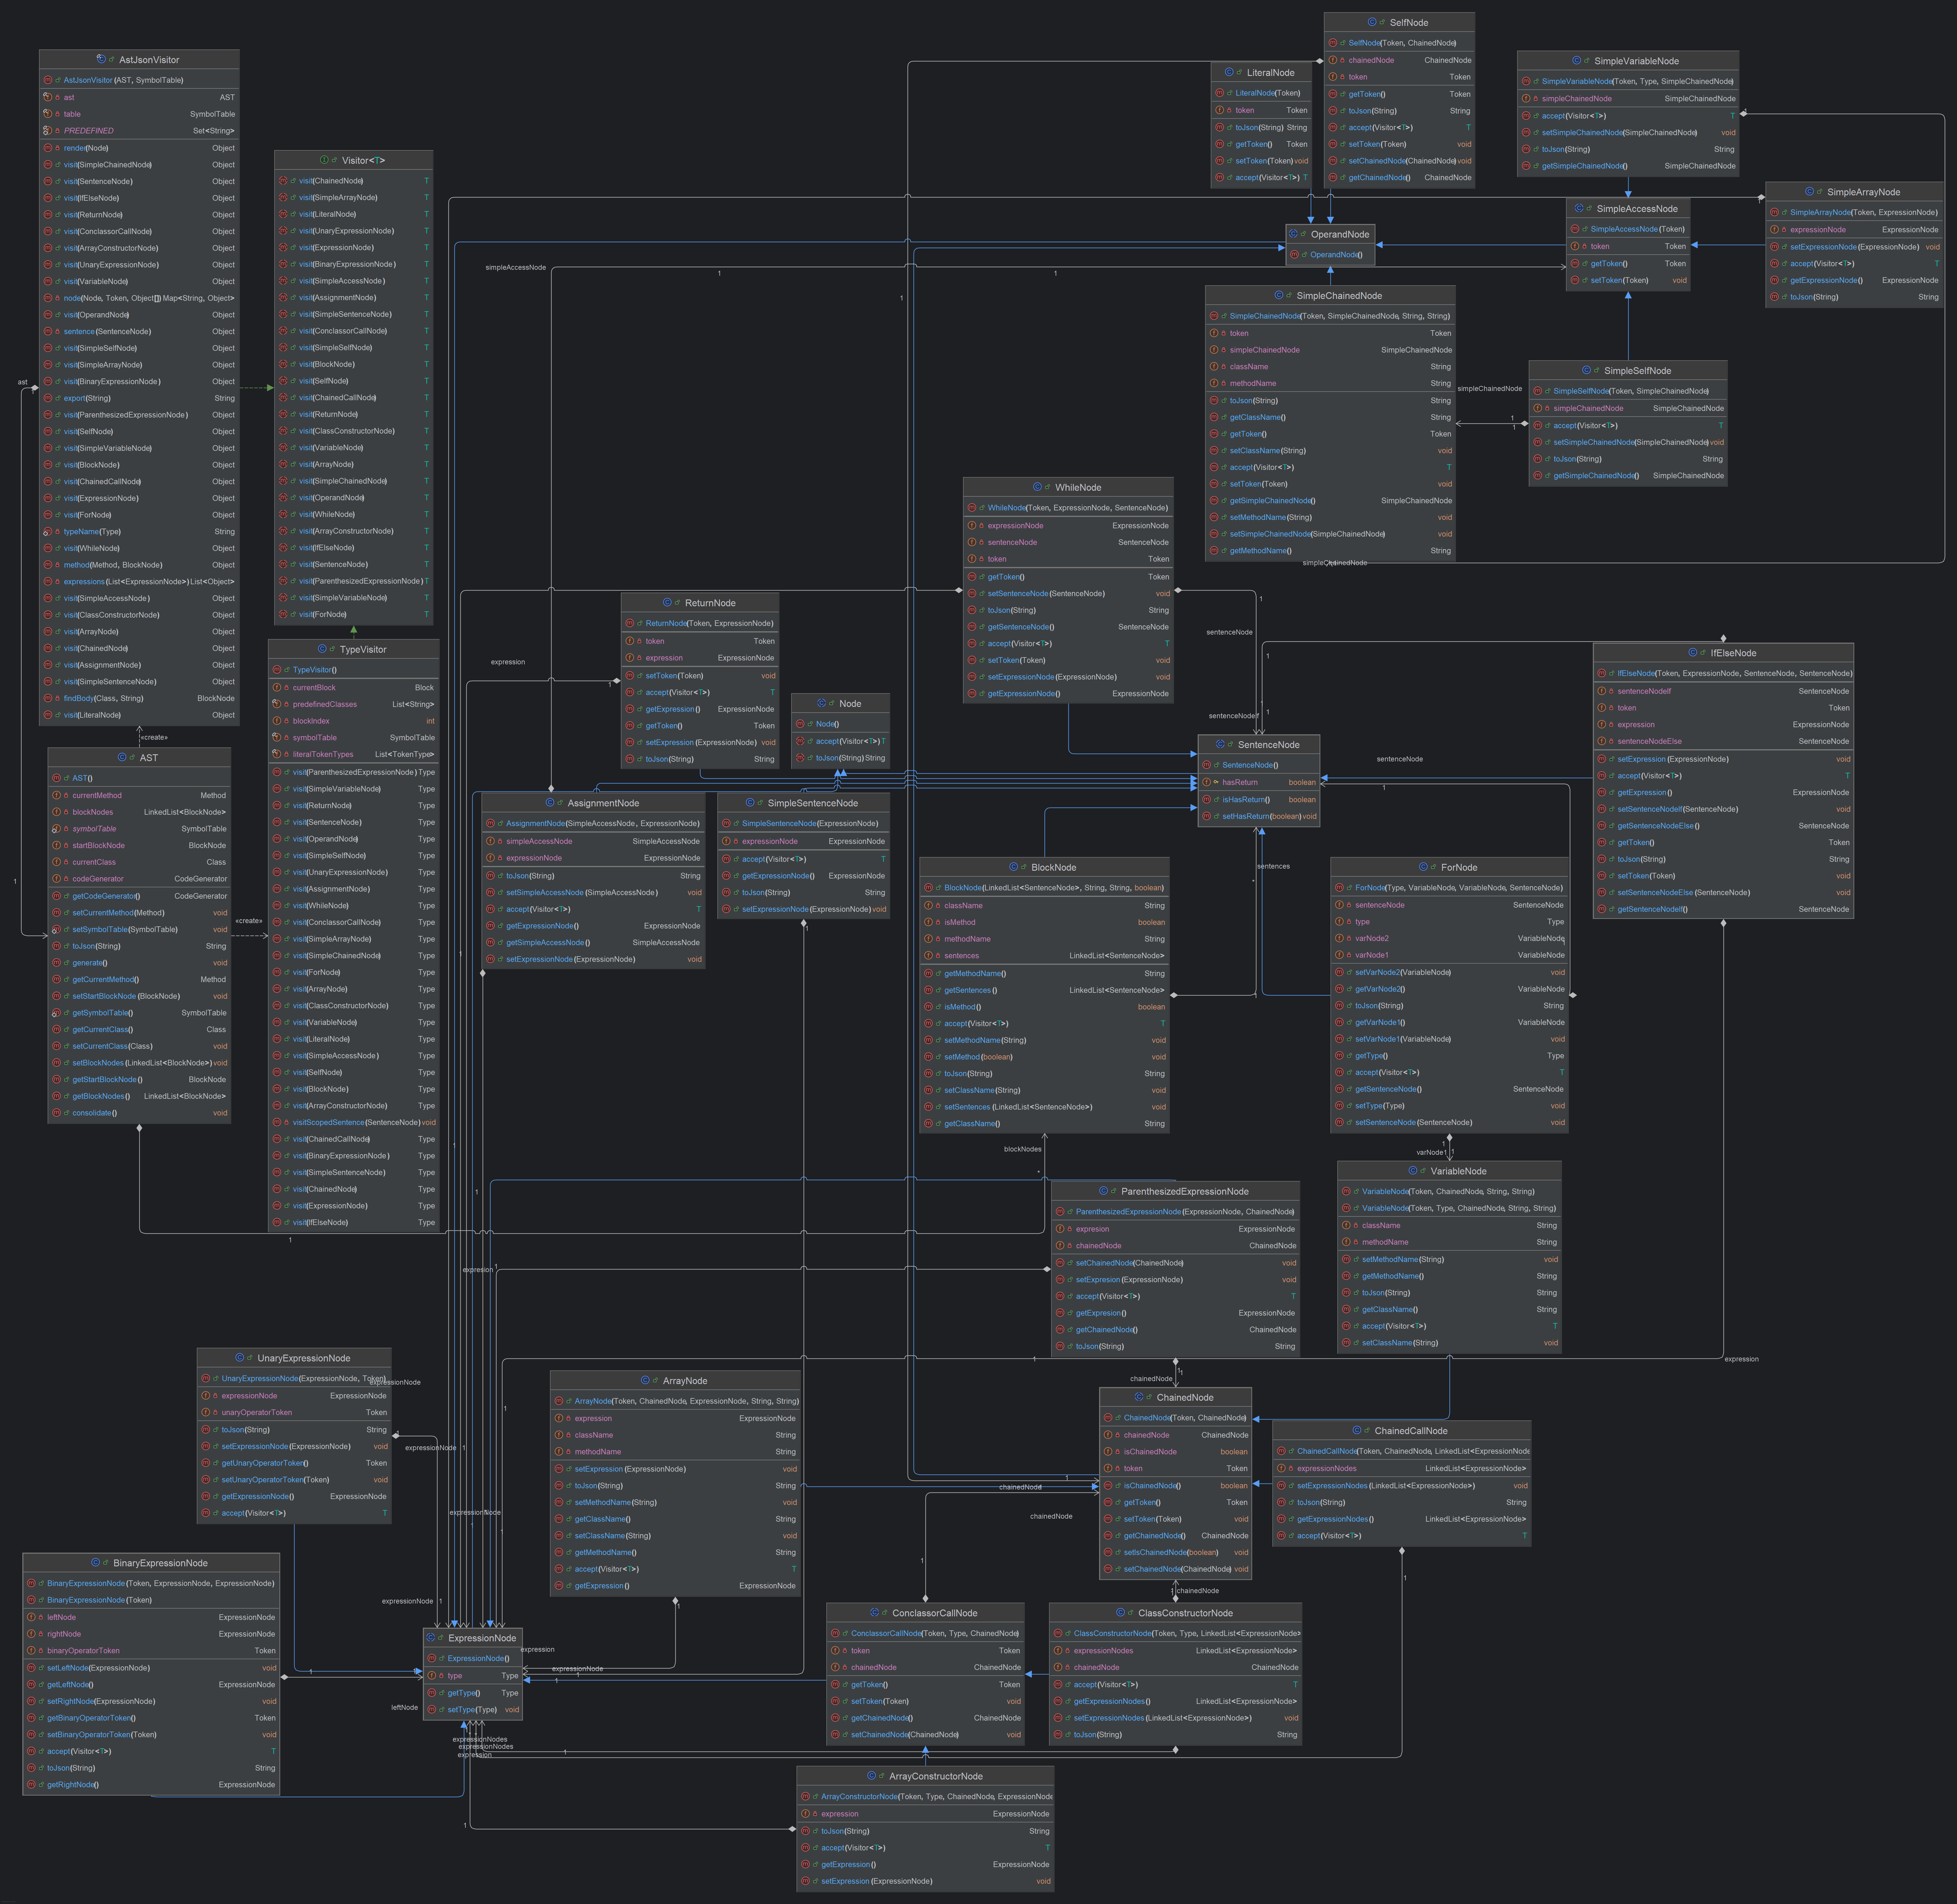
\includegraphics[width=\linewidth,height=0.9\textheight,keepaspectratio]{diagramas/UML_AST.png}
  \caption{Diagrama de clases del AST.}
  \label{fig:uml-ast}
\end{figure}
\clearpage

% Diagramas vectoriales: las flechas con triangulo apuntan a la superclase.
\begin{figure}[H]
\centering
\resizebox{\linewidth}{!}{%
\begin{tikzpicture}[
  box/.style={draw,rectangle,align=center,font=\footnotesize\ttfamily,text width=5.2cm,inner sep=6pt},
  inh/.style={-{Triangle[open,length=6pt,width=7pt]}},
  dep/.style={dashed,-{Stealth[length=5pt]}}]
\node[box] (ast) at (-3,0) {\textbf{AST}\\\rule{4.4cm}{0.3pt}\\
blockNodes:\\LinkedList<BlockNode>\\startBlockNode: BlockNode\\symbolTable (static):\\SymbolTable\\\rule{4.4cm}{0.3pt}\\
consolidate()\\toJson(indent): String};
\node[box] (node) at (3,0) {\textit{Node}\\\rule{4.4cm}{0.3pt}\\
accept(visitor): T\\toJson(indent): String};
\node[box,below=1.1cm of ast] (block) {\textbf{BlockNode}\\\rule{4.4cm}{0.3pt}\\
sentences:\\LinkedList<SentenceNode>\\className: String\\methodName: String\\isMethod: boolean};
\node[box,right=0.8cm of block] (sentence) {\textit{SentenceNode}\\\rule{4.4cm}{0.3pt}\\
hasReturn: boolean};
\node[box,below=0.8cm of sentence] (expression) {\textit{ExpressionNode}\\\rule{4.4cm}{0.3pt}\\ type: Type};
\node[box,below=0.9cm of block] (visitor) {\textit{Visitor<T>}\\\rule{4.4cm}{0.3pt}\\ visit(tipoDeNodo): T};
\node[box,below=1cm of visitor,xshift=-3.1cm] (types) {\textbf{TypeVisitor}\\\rule{4.4cm}{0.3pt}\\ Visitor<Type>\\chequeo semántico};
\node[box,below=1cm of visitor,xshift=3.1cm] (json) {\textbf{AstJsonVisitor}\\\rule{4.4cm}{0.3pt}\\ Visitor<Object>\\export(indent): String};
\draw[inh] (sentence) -- (node);
\draw[inh] (expression.east) -- ++(0.5,0) |- (node.east);
\draw[inh] (block.east) -- (sentence.west);
\draw[-{Diamond[open,length=8pt,width=6pt]}] (block.north) -- node[left,font=\small] { } (ast.south);
\draw[dep] (node.west) -- ++(-0.3,0) |- (visitor.east);
\draw[inh,dashed] (types.north) -- (visitor.south);
\draw[inh,dashed] (json.north) -- (visitor.south);
\end{tikzpicture}}
\caption{AST, nodos base y visitantes.}
\label{fig:ast-base}
\end{figure}

\begin{figure}[H]
\centering
\resizebox{0.95\linewidth}{!}{%
\begin{tikzpicture}[
  box/.style={draw,rectangle,align=center,font=\small,text width=5.8cm,inner sep=5pt},
  inh/.style={-{Triangle[open,length=6pt,width=7pt]}}]
\node[box,text width=3.5cm] (root) at (-3.8,-5.4) {\textit{SentenceNode}\\hasReturn: boolean};
\node[box] (b) at (3.8,0) {\textbf{BlockNode}\\lista ordenada, contexto, isMethod};
\node[box] (a) at (3.8,-1.8) {\textbf{AssignmentNode}\\acceso de destino, expresión de origen};
\node[box] (s) at (3.8,-3.6) {\textbf{SimpleSentenceNode}\\expresión};
\node[box] (i) at (3.8,-5.4) {\textbf{IfElseNode}\\token, condición, rama if, rama else};
\node[box] (w) at (3.8,-7.2) {\textbf{WhileNode}\\token, condición, cuerpo};
\node[box] (f) at (3.8,-9) {\textbf{ForNode}\\tipo, variable, iterable, cuerpo};
\node[box] (r) at (3.8,-10.8) {\textbf{ReturnNode}\\token, expresión opcional};
\draw (0,0) -- (0,-10.8);
\draw[inh] (0,-5.4) -- (root.east);
\foreach \n in {b,a,s,i,w,f,r} {\draw (\n.west) -- (0,0 |- \n.west);}
\end{tikzpicture}}
\caption{Jerarquía de sentencias y referencias que conserva cada nodo.}
\label{fig:ast-sentencias}
\end{figure}

\begin{figure}[H]
\centering
\resizebox{\linewidth}{!}{%
\begin{tikzpicture}[
  box/.style={draw,rectangle,align=center,font=\small,text width=4.8cm,inner sep=5pt},
  inh/.style={-{Triangle[open,length=6pt,width=7pt]}}]
\node[box,text width=3.7cm] (exp) at (-4.4,-2.5) {\textit{ExpressionNode}\\type: Type};
\node[box] (bin) at (2,0) {BinaryExpressionNode};
\node[box] (un) at (2,-1.25) {UnaryExpressionNode};
\node[box] (par) at (2,-2.5) {Parenthesized\\ExpressionNode};
\node[box] (con) at (2,-3.75) {\textit{ConclassorCallNode}};
\node[box] (op) at (2,-5) {\textit{OperandNode}};
\draw (-1.2,0) -- (-1.2,-5);
\draw[inh] (-1.2,-2.5) -- (exp.east);
\foreach \n in {bin,un,par,con,op} {\draw (\n.west) -- (-1.2,0 |- \n.west);}
\node[box] (obj) at (8,-3.15) {ClassConstructorNode};
\node[box] (arr) at (8,-4.4) {ArrayConstructorNode};
\draw[inh] (obj.west) -- (con.east);
\draw[inh] (arr.west) -- (con.east);
\end{tikzpicture}}
\caption{Expresiones, operadores y nodos de construcción de objetos y arreglos.}
\label{fig:ast-expresiones}
\end{figure}

\begin{figure}[H]
\centering
\resizebox{\linewidth}{!}{%
\begin{tikzpicture}[
  box/.style={draw,rectangle,align=center,font=\small,text width=4.6cm,inner sep=5pt},
  inh/.style={-{Triangle[open,length=6pt,width=7pt]}}]
\node[box,text width=3cm] (op) at (-5,-3) {\textit{OperandNode}};
\node[box] (lit) at (0,0) {LiteralNode};
\node[box] (self) at (0,-1.4) {SelfNode};
\node[box] (simplechain) at (0,-2.8) {SimpleChainedNode};
\node[box] (simple) at (0,-4.2) {\textit{SimpleAccessNode}};
\node[box] (chain) at (0,-8.2) {\textit{ChainedNode}};
\draw (-3,0) -- (-3,-8.2);
\draw[inh] (-3,-3) -- (op.east);
\foreach \n in {lit,self,simplechain,simple,chain} {\draw (\n.west) -- (-3,0 |- \n.west);}
\node[box] (sv) at (6,-3.2) {SimpleVariableNode};
\node[box] (ss) at (6,-4.6) {SimpleSelfNode};
\node[box] (sa) at (6,-6) {SimpleArrayNode};
\foreach \n in {sv,ss,sa} {\draw[inh] (\n.west) -- (simple.east);}
\node[box] (v) at (6,-7.6) {VariableNode};
\node[box] (ar) at (6,-9) {ArrayNode};
\node[box] (call) at (6,-10.4) {ChainedCallNode};
\foreach \n in {v,ar,call} {\draw[inh] (\n.west) -- (chain.east);}
\end{tikzpicture}}
\caption{Jerarquía de operandos, destinos de asignación y accesos encadenados.}
\label{fig:ast-accesos}
\end{figure}


\subsection{Información almacenada y operaciones}
\lexcode{Node} define \lexcode{accept(Visitor<T>)} y
\lexcode{toJson(String)}.
\lexcode{ExpressionNode} agrega el atributo \texttt{type} y
\lexcode{SentenceNode} agrega \texttt{hasReturn}.

\lexcode{AST.consolidate()} visita primero los bloques de métodos y
constructores, y luego \texttt{start}. \lexcode{AST.toJson()} utiliza
el exportador del árbol completo.

La tabla siguiente detalla los datos propios de cada clase; los atributos
heredados se obtienen de la jerarquía de los diagramas.
\begingroup
\small
\renewcommand{\arraystretch}{1.2}
\setlength{\tabcolsep}{5pt}
\setlength{\LTleft}{0pt}
\setlength{\LTright}{0pt}
\begin{longtable}{|>{\raggedright\arraybackslash}p{0.35\textwidth}|>{\raggedright\arraybackslash}p{\dimexpr0.65\textwidth-4\tabcolsep-3\arrayrulewidth\relax}|}
\caption{Datos conservados por los nodos del AST}\label{tab:nodos-ast}\\
\hline
\textbf{Clase} & \textbf{Estructura} \\ \hline
\endfirsthead
\hline
\textbf{Clase} & \textbf{Estructura} \\ \hline
\endhead
\texttt{Node} & Raíz abstracta. Operaciones accept(visitor) y toJson(indent). \\ \hline
\texttt{Assignment\allowbreak Node} & \texttt{simple\allowbreak Access\allowbreak Node}: \texttt{Simple\allowbreak Access\allowbreak Node}\newline \texttt{expression\allowbreak Node}: \texttt{Expression\allowbreak Node} \\ \hline
\texttt{Block\allowbreak Node} & \texttt{sentences}: \texttt{Linked\allowbreak List<Sentence\allowbreak Node>}\newline \texttt{class\allowbreak Name}: \texttt{String}\newline \texttt{method\allowbreak Name}: \texttt{String}\newline \texttt{is\allowbreak Method}: \texttt{boolean} \\ \hline
\texttt{For\allowbreak Node} & \texttt{type}: \texttt{Type}\newline \texttt{var\allowbreak Node1}: \texttt{Variable\allowbreak Node}\newline \texttt{var\allowbreak Node2}: \texttt{Variable\allowbreak Node}\newline \texttt{sentence\allowbreak Node}: \texttt{Sentence\allowbreak Node} \\ \hline
\texttt{If\allowbreak Else\allowbreak Node} & \texttt{token}: \texttt{Token}\newline \texttt{expression}: \texttt{Expression\allowbreak Node}\newline \texttt{sentence\allowbreak Node\allowbreak If}: \texttt{Sentence\allowbreak Node}\newline \texttt{sentence\allowbreak Node\allowbreak Else}: \texttt{Sentence\allowbreak Node} \\ \hline
\texttt{Return\allowbreak Node} & \texttt{token}: \texttt{Token}\newline \texttt{expression}: \texttt{Expression\allowbreak Node} \\ \hline
\texttt{Sentence\allowbreak Node} & \texttt{has\allowbreak Return}: \texttt{boolean} \\ \hline
\texttt{Simple\allowbreak Sentence\allowbreak Node} & \texttt{expression\allowbreak Node}: \texttt{Expression\allowbreak Node} \\ \hline
\texttt{While\allowbreak Node} & \texttt{expression\allowbreak Node}: \texttt{Expression\allowbreak Node}\newline \texttt{sentence\allowbreak Node}: \texttt{Sentence\allowbreak Node}\newline \texttt{token}: \texttt{Token} \\ \hline
\texttt{Array\allowbreak Constructor\allowbreak Node} & \texttt{expression}: \texttt{Expression\allowbreak Node} \\ \hline
\texttt{Array\allowbreak Node} & \texttt{expression}: \texttt{Expression\allowbreak Node}\newline \texttt{class\allowbreak Name}: \texttt{String}\newline \texttt{method\allowbreak Name}: \texttt{String} \\ \hline
\texttt{Binary\allowbreak Expression\allowbreak Node} & \texttt{left\allowbreak Node}: \texttt{Expression\allowbreak Node}\newline \texttt{right\allowbreak Node}: \texttt{Expression\allowbreak Node}\newline \texttt{binary\allowbreak Operator\allowbreak Token}: \texttt{Token} \\ \hline
\texttt{Chained\allowbreak Call\allowbreak Node} & \texttt{expression\allowbreak Nodes}: \texttt{Linked\allowbreak List<Expression\allowbreak Node>} \\ \hline
\texttt{Chained\allowbreak Node} & \texttt{token}: \texttt{Token}\newline \texttt{chained\allowbreak Node}: \texttt{Chained\allowbreak Node}\newline \texttt{is\allowbreak Chained\allowbreak Node}: \texttt{boolean} \\ \hline
\texttt{Class\allowbreak Constructor\allowbreak Node} & \texttt{expression\allowbreak Nodes}: \texttt{Linked\allowbreak List<Expression\allowbreak Node>}\newline \texttt{chained\allowbreak Node}: \texttt{Chained\allowbreak Node} \\ \hline
\texttt{Conclassor\allowbreak Call\allowbreak Node} & \texttt{token}: \texttt{Token}\newline \texttt{chained\allowbreak Node}: \texttt{Chained\allowbreak Node} \\ \hline
\texttt{Expression\allowbreak Node} & \texttt{type}: \texttt{Type} \\ \hline
\texttt{Literal\allowbreak Node} & \texttt{token}: \texttt{Token} \\ \hline
\texttt{Operand\allowbreak Node} & No agrega campos propios. \\ \hline
\texttt{Parenthesized\allowbreak Expression\allowbreak Node} & \texttt{expresion}: \texttt{Expression\allowbreak Node}\newline \texttt{chained\allowbreak Node}: \texttt{Chained\allowbreak Node} \\ \hline
\texttt{Self\allowbreak Node} & \texttt{chained\allowbreak Node}: \texttt{Chained\allowbreak Node}\newline \texttt{token}: \texttt{Token} \\ \hline
\texttt{Simple\allowbreak Access\allowbreak Node} & \texttt{token}: \texttt{Token} \\ \hline
\texttt{Simple\allowbreak Array\allowbreak Node} & \texttt{expression\allowbreak Node}: \texttt{Expression\allowbreak Node} \\ \hline
\texttt{Simple\allowbreak Chained\allowbreak Node} & \texttt{token}: \texttt{Token}\newline \texttt{simple\allowbreak Chained\allowbreak Node}: \texttt{Simple\allowbreak Chained\allowbreak Node}\newline \texttt{class\allowbreak Name}: \texttt{String}\newline \texttt{method\allowbreak Name}: \texttt{String} \\ \hline
\texttt{Simple\allowbreak Self\allowbreak Node} & \texttt{simple\allowbreak Chained\allowbreak Node}: \texttt{Simple\allowbreak Chained\allowbreak Node} \\ \hline
\texttt{Simple\allowbreak Variable\allowbreak Node} & \texttt{simple\allowbreak Chained\allowbreak Node}: \texttt{Simple\allowbreak Chained\allowbreak Node} \\ \hline
\texttt{Unary\allowbreak Expression\allowbreak Node} & \texttt{unary\allowbreak Operator\allowbreak Token}: \texttt{Token}\newline \texttt{expression\allowbreak Node}: \texttt{Expression\allowbreak Node} \\ \hline
\texttt{Variable\allowbreak Node} & \texttt{class\allowbreak Name}: \texttt{String}\newline \texttt{method\allowbreak Name}: \texttt{String} \\ \hline
\end{longtable}
\endgroup


\section{Estrategias de chequeo semántico}
\label{sec:chequeos-sentencias}

\subsection{Literales, operadores y asignaciones}
\begin{description}[style=nextline]
  \item[Literal]
  \lexcode{visit(LiteralNode)} admite las categorías de literal entero,
  cadena, booleano y \texttt{nil}. El tipo conserva la categoría del
  token; \lexcode{Type.getTypeName()} presenta los nombres
  \texttt{Int}, \texttt{Str} y \texttt{Bool} para sus constantes.
  \item[Operación binaria]
  Se visitan los dos operandos antes de comprobar el operador.
  Las operaciones aritméticas exigen \texttt{Int}; las lógicas exigen
  \texttt{Bool}; las relacionales exigen \texttt{Int} y devuelven
  \texttt{Bool}. La igualdad y desigualdad utilizan la operación común
  de compatibilidad y devuelven \texttt{Bool}.
  \item[Operación unaria]
  Los operadores \texttt{+}, \texttt{-}, \texttt{++} y \texttt{--}
  exigen un operando entero. El operador \texttt{!} exige un booleano.
  El incremento y decremento rechazan un operando que sea directamente
  un \lexcode{LiteralNode}. La comprobación del tipo utiliza el tipo
  almacenado en el hijo, visitándolo antes si todavía no lo tiene.
  \item[Asignación]
  Se visita el acceso del lado izquierdo y la expresión del derecho.
  Ambos tipos se guardan en los nodos y se comparan mediante
  \lexcode{Type.areCompatible()}. La incompatibilidad se informa en el
  token del acceso de destino.
\end{description}

\begin{center}
\small
\begin{tabular}{|l|l|l|}
\hline
\textbf{Operadores} & \textbf{Operandos requeridos} & \textbf{Resultado} \\ \hline
\texttt{+ - * /} binarios & \texttt{Int}, \texttt{Int} & \texttt{Int} \\ \hline
\texttt{\&\& ||} & \texttt{Bool}, \texttt{Bool} & \texttt{Bool} \\ \hline
\texttt{< > <= >=} & \texttt{Int}, \texttt{Int} & \texttt{Bool} \\ \hline
\texttt{== !=} & Tipos compatibles & \texttt{Bool} \\ \hline
\texttt{+ - ++ --} unarios & \texttt{Int} & \texttt{Int} \\ \hline
\texttt{!} & \texttt{Bool} & \texttt{Bool} \\ \hline
\end{tabular}
\end{center}

\subsection{Arreglos y recorridos}
\lexcode{ArrayNode} y \lexcode{SimpleArrayNode} comprueban que el
índice sea entero y que el identificador resuelto tenga tipo
\lexcode{ArrayType}. El tipo del acceso es el subtipo de los elementos.
Una asignación a un elemento se comprueba después contra ese subtipo.

\lexcode{visit(ForNode)} obtiene el tipo del identificador que se
recorre, exige un arreglo y compara el tipo de su elemento con el tipo
declarado para la variable de iteración. Luego visita el cuerpo en su
ámbito. Los límites de los índices y los valores nulos corresponden
a controles durante la ejecución del código generado.

\subsection{Llamadas, encadenados y visibilidad}
\begin{description}[style=nextline]
  \item[Llamada a método]
  Se busca el nombre en la clase receptora y su jerarquía. Primero se
  compara la cantidad de argumentos, si coincide, se visitan sus
  expresiones y se comparan los tipos con los parámetros formales en
  orden. El resultado de la llamada es el tipo de retorno del método.
  \item[Llamada a constructor]
  Se obtiene el constructor de la clase y se compara la cantidad y los
  tipos de argumentos. El nodo conserva como tipo el de la clase creada.
  Las posiciones de argumentos de los diagnósticos comienzan en cero.
  \item[Acceso estático o de instancia]
  El acceso a través del nombre de clase exige un método estático.
  El recorrido a través de una variable receptora rechaza la llamada
  a un método estático mediante una instancia.
  \item[Encadenado]
  El tipo del receptor determina la clase donde se busca el siguiente
  miembro. Se rechaza continuar un acceso sobre el retorno
  \texttt{void}, y se comprueban los accesos a miembros que no existen
  y los encadenados incompatibles sobre tipos primitivos.
  \item[Atributo público o privado]
  Los visitantes consultan la visibilidad y la clase que declaró el
  atributo. El acceso externo a un atributo privado se rechaza, al igual
  que los accesos privados heredados cubiertos por las pruebas.
  \item[Uso de self]
  Los nodos \lexcode{SelfNode} y \lexcode{SimpleSelfNode} comprueban
  el contexto del método al recorrer un acceso encadenado y rechazan
  ese uso de \texttt{self} en un método estático.
\end{description}

\subsection{Condiciones y retornos}
Las condiciones de \texttt{if} y \texttt{while} se visitan y deben
tener tipo \texttt{Bool}. Cada rama o cuerpo se recorre dentro del
ámbito correspondiente.

En \lexcode{visit(ReturnNode)} se obtiene el tipo de la expresión y
se compara con el retorno declarado del método actual. Un retorno válido
marca \texttt{hasReturn}. Al cerrar un bloque raíz de método no \texttt{void},
se exige que la marca esté establecida. Los constructores se excluyen
del control de retorno faltante.

\subsection{Decisiones de representación}
\label{sec:limites-sentencias}
\begin{description}[style=nextline]
  \item[Sentencias vacías]
  El punto y coma aislado se conserva como una entrada nula en la lista
  del bloque. El exportador la representa con
  \lexcode{{"nodeType": "EmptySentence"}}. Una rama vacía puede
  envolverse en un bloque vacío para conservar su ámbito.
  \item[Compatibilidad de tipos]
  Se compara categorías de token y se admite
  equivalencias entre constantes y clases primitivas. Para Arrays, se
  compara las categorías de sus elementos; no almacena la longitud
  como parte de \lexcode{ArrayType} ya que se define en tiempo de ejecución.
  \item[Retorno dentro de ciclos]
  Los visitantes de \texttt{while} y \texttt{for} propagan la marca
  de retorno de su bloque. 
\end{description}

\section{Errores de sentencias}
\label{sec:errores-sentencias}
El análisis se interrumpe con la primera excepción: no se recupera ni se
continúa con las sentencias posteriores. \lexcode{ASTException} hereda
de \lexcode{SemanticException}. Los conflictos de búsqueda pueden
provenir también de las excepciones de tabla de símbolos.

\begin{description}[style=nextline]
  \item[Tipos incompatibles]
  \lexcode{TypeMismatchException}: asignaciones, operadores, condiciones,
  índices o recorridos con tipos distintos de los esperados.
  \item[Retorno incorrecto o ausente]
  \lexcode{InvalidReturnException} compara el retorno encontrado con el
  declarado. \lexcode{MissingReturnException} señala un método con
  resultado cuyo bloque no quedó marcado con retorno.
  \item[Argumentos de métodos y constructores]
  \texttt{Invalid\allowbreak Method\allowbreak Argument\allowbreak Count\allowbreak Exception} e
  \texttt{Invalid\allowbreak Constructor\allowbreak Arguments\allowbreak Count\allowbreak Exception} informan diferencias
  de cantidad. \texttt{Invalid\allowbreak Method\allowbreak Argument\allowbreak Type\allowbreak Exception} y
  \texttt{Invalid\allowbreak Constructor\allowbreak Argument\allowbreak Type\allowbreak Exception} informan el índice y
  los tipos del argumento incompatible.
  \item[Acceso inválido]
  \texttt{Invalid\allowbreak Attribute\allowbreak Access\allowbreak Exception},
  \texttt{Invalid\allowbreak Method\allowbreak Access\allowbreak Exception},
  \lexcode{InvalidVoidAccessException} e
  \texttt{Invalid\allowbreak Primitive\allowbreak Access\allowbreak Exception} cubren visibilidad y
  encadenados. Las búsquedas también pueden producir
  \texttt{Local\allowbreak Variable\allowbreak Not\allowbreak Found\allowbreak Exception},
  \lexcode{MethodNotFoundException},
  \lexcode{AttributeNotFoundException} o
  \lexcode{ClassNotFoundException}.
  \item[Contexto estático]
  \texttt{Non\allowbreak Static\allowbreak Method\allowbreak Called\allowbreak From\allowbreak Class\allowbreak Exception},
  \texttt{Static\allowbreak Method\allowbreak Called\allowbreak From\allowbreak Instance\allowbreak Exception} y
  \texttt{Self\allowbreak Used\allowbreak In\allowbreak Static\allowbreak Mehthod\allowbreak Exception} corresponden a las formas de
  acceso estático y al uso de \texttt{self}. Los nombres conservan la
  escritura de las clases Java.
  \item[Operación sobre literal o conflicto de iteración]
  \texttt{Invalid\allowbreak Literal\allowbreak Operation\allowbreak Exception} rechaza el incremento o
  decremento directo de un literal.
  \texttt{Variable\allowbreak Redeclaration\allowbreak In\allowbreak For\allowbreak Loop\allowbreak Exception} señala un conflicto
  de la variable de iteración con el método que la contiene.
\end{description}

El ejecutador muestra \texttt{ERROR: SEMANTICO - SENTENCIAS} y el
diagnóstico sin la traza de llamadas de Java. Los errores detectados en
la lectura previa conservan el encabezado de declaraciones, léxico o
sintáctico que corresponda. Por ejemplo,
\lexcode{tc/etapa4/error/returnIncompatible.s} produce:
\lstinputlisting[style=bnftinys]{ejemplos/sentencias/returnIncompatible.salida.txt}

Cuando falla el análisis no se escriben nuevos JSON. Los archivos de
ejecuciones anteriores permanecen en el directorio. Una vez completado
el análisis, la escritura de los dos archivos no es transaccional.

\section{Formato de exportación del AST}
\label{sec:json-sentencias}
\lexcode{AstJsonVisitor.export()} recorre las clases de la tabla e
incluye las entradas de usuario y las predefinidas. La raíz del JSON
tiene dos propiedades: \texttt{classes} y \texttt{startMethod}.
\begin{description}[style=nextline]
  \item[Clase]
  Contiene \texttt{name}, \texttt{parent}, \texttt{predefined},
  \texttt{attributes}, \texttt{constructor} y \texttt{methods}.
  Cada atributo incluye nombre, tipo y visibilidad.
  \item[Método o constructor]
  Contiene \texttt{name}, \texttt{returnType}, \texttt{static},
  \texttt{parameters}, \texttt{variables} y \texttt{body}.
  Los parámetros y variables conservan sus posiciones.
  \item[Sentencia o expresión]
  La propiedad \texttt{nodeType} identifica la clase concreta del nodo.
  Sus propiedades anidadas conservan los hijos y permiten observar la
  estructura del árbol. Si el nodo tiene token, se agregan
  \texttt{lexeme}, \texttt{row} y \texttt{column}; si una expresión
  tiene tipo calculado, también se agrega \texttt{type}.
  \item[Orden de los cuerpos]
  \texttt{BlockNode.sentences} es un arreglo que conserva el orden del
  fuente. Los nodos binarios tienen \texttt{left} y \texttt{right};
  las llamadas, \texttt{arguments} y \texttt{chained}; los condicionales,
  \texttt{condition}, \texttt{then} y \texttt{else}; los ciclos,
  su condición o iterable y \texttt{body}.
\end{description}

Los métodos predefinidos tienen \texttt{body: null} porque sus cuerpos
pertenecen al entorno de ejecución. Para un método heredado, el
exportador busca el bloque por nombre en la clase y continúa por los
padres hasta encontrar su cuerpo. Una alternativa \texttt{else}
ausente se exporta como \texttt{null}. Los caracteres especiales de
las cadenas se escapan mediante \lexcode{JsonWriter}.

\clearpage
\subsection{Ejemplo: lectura de un atributo público heredado}
\lstinputlisting[style=bnftinys]{../tc/etapa4/success/accesoAtributoPublicoHerenciaLectura.s}

Y su salida JSON correspondiente:
\lstinputlisting[style=bnftinys,basicstyle=\ttfamily\footnotesize]{ejemplos/sentencias/accesoAtributoPublicoHerenciaLectura.ast.json}

\clearpage
\section{Escenarios y casos de prueba}
\label{sec:casos-sentencias}

\subsection{Casos que deben aceptarse}
Se espera finalizar el chequeo de sentencias sin excepciones.
La ejecución mediante \lexcode{Etapa4} debe producir los dos JSON.
\begingroup
\small
\renewcommand{\arraystretch}{1.2}
\setlength{\tabcolsep}{5pt}
\setlength{\LTleft}{0pt}
\setlength{\LTright}{0pt}
\begin{longtable}{|>{\raggedright\arraybackslash}p{0.40\textwidth}|>{\raggedright\arraybackslash}p{0.28\textwidth}|>{\raggedright\arraybackslash}p{\dimexpr0.32\textwidth-6\tabcolsep-4\arrayrulewidth\relax}|}
\caption{Casos válidos del chequeo de sentencias}\label{tab:sentencias-success}\\
\hline
\textbf{Archivo} & \textbf{Propósito} & \textbf{Resultado esperado} \\ \hline
\endfirsthead
\hline
\textbf{Archivo} & \textbf{Propósito} & \textbf{Resultado esperado} \\ \hline
\endhead
\texttt{acceso\allowbreak Atributo\allowbreak Publico\allowbreak Herencia\allowbreak Lectura.s} & Leer un atributo público heredado dentro de un método. & Aceptar valor heredado, su asignación a copia y el retorno Int. \\ \hline
\texttt{acceso\allowbreak Atributo\allowbreak Publico\allowbreak Herencia\allowbreak Parametro.s} & Usar un atributo público heredado como argumento. & Aceptar self.valor como argumento Int de IO.out\_int. \\ \hline
\texttt{acceso\allowbreak Atributo\allowbreak Publico\allowbreak Lectura.s} & Leer un atributo público desde una variable receptora. & Aceptar caja.valor como origen de una asignación Int. \\ \hline
\texttt{acceso\allowbreak Atributo\allowbreak Publico\allowbreak Parametro.s} & Pasar un atributo público como argumento. & Aceptar caja.valor al llamar a IO.out\_int. \\ \hline
\texttt{array.s} & Crear, escribir y leer un arreglo entero. & Aceptar índices Int y la suma de elementos Int. \\ \hline
\texttt{array\allowbreak In\allowbreak Method.s} & Usar arreglos en atributos, parámetros y retornos de elementos. & Aceptar datos, arr y las operaciones sobre sus elementos. \\ \hline
\texttt{array\allowbreak Operations.s} & Combinar accesos a elementos en una expresión. & Aceptar la suma entera usada como argumento de salida. \\ \hline
\texttt{array\allowbreak Tamanio\allowbreak Dinamico.s} & Crear un arreglo con una expresión de longitud variable. & Aceptar new Int[n] en el recorrido actual. \\ \hline
\texttt{bloque\allowbreak Valido.s} & Comprobar una operación con parámetro y variable local. & Aceptar x por 2, la asignación a resultado y el retorno Int. \\ \hline
\texttt{boolean\allowbreak And\allowbreak Comparison\allowbreak Types.s} & Combinar precedencia aritmética, comparación y conjunción. & Aceptar el resultado Bool y las condiciones de if y while. \\ \hline
\texttt{boolean\allowbreak Operations.s} & Retornar comparaciones desde métodos Bool. & Aceptar las comparaciones de enteros y sus llamadas. \\ \hline
\texttt{chained\allowbreak Methods.s} & Encadenar atributo de objeto y llamada a método. & Aceptar b.miA.saludo() y su resultado Str. \\ \hline
\texttt{class\allowbreak Attributes.s} & Procesar cuerpos vacíos con atributos declarados. & Aceptar constructor, método y start vacíos. \\ \hline
\texttt{class\allowbreak Equal.s} & Comparar referencias del mismo tipo. & Aceptar x == y y asignar su resultado a Bool. \\ \hline
\texttt{class\allowbreak Method.s} & Procesar parámetros, variables locales y varias implementaciones. & Aceptar sus cuerpos vacíos después de consolidar A. \\ \hline
\texttt{complex\allowbreak Expression.s} & Comprobar aritmética con precedencia y argumentos. & Aceptar el retorno Int de calcular y su asignación a resultado. \\ \hline
\texttt{constructor\allowbreak Array.s} & Crear arreglos de tipos primitivos. & Aceptar Array Int, Array Str y Array Bool con sus creaciones. \\ \hline
\texttt{for\allowbreak Anidado.s} & Resolver variables en recorridos anidados. & Aceptar j en su cuerpo e i después del recorrido interior. \\ \hline
\texttt{for\allowbreak Inside\allowbreak Method.s} & Recorrer un parámetro arreglo dentro de un método. & Aceptar el iterador Int y la llamada a procesar. \\ \hline
\texttt{for\allowbreak With\allowbreak If.s} & Combinar ámbito de for y condición if. & Aceptar i en la comparación y en el cuerpo del condicional. \\ \hline
\texttt{if\&else.s} & Comprobar condiciones y llamadas en ramas sin llaves. & Aceptar comparaciones Bool y argumentos Str. \\ \hline
\texttt{inheritance\allowbreak Chain.s} & Recorrer cuerpos vacíos después de consolidar herencia. & Aceptar los constructores de A, B, C y D y start vacío. \\ \hline
\texttt{inherited\allowbreak Public\allowbreak Attribute.s} & Escribir un atributo heredado e invocar un método heredado. & Aceptar b.x y b.getX() con resultado Int. \\ \hline
\texttt{literals.s} & Asignar constantes a tipos primitivos. & Aceptar las asignaciones Int, Bool y Str. \\ \hline
\texttt{merge\allowbreak Class.s} & Comprobar cuerpos con herencia y partes de una clase. & Aceptar operaciones Int y el retorno de un arreglo declarado. \\ \hline
\texttt{method\allowbreak Arguments\allowbreak Correct.s} & Comprobar argumentos y llamadas anidadas. & Aceptar dos argumentos Int en cada llamada a sumar. \\ \hline
\texttt{methods\&Attributes.s} & Comprobar métodos distribuidos y acceso a atributos propios. & Aceptar las asignaciones y el retorno entero de m3. \\ \hline
\texttt{methods.s} & Comprobar un retorno de atributo propio. & Aceptar self.i1 como resultado Int de m3. \\ \hline
\texttt{object\allowbreak Methods.s} & Combinar construcción, actualización y lectura de un objeto. & Aceptar el incremento de valor y las llamadas de instancia. \\ \hline
\texttt{print\allowbreak For.s} & Recorrer un arreglo y usar el iterador como argumento. & Aceptar el iterador Int al llamar a IO.out\_int. \\ \hline
\texttt{prints.s} & Invocar métodos predefinidos con argumentos compatibles. & Aceptar IO.out\_str con Str e IO.out\_int con Int. \\ \hline
\texttt{public\allowbreak Attributes.s} & Actualizar un atributo público y obtenerlo por un método. & Aceptar p.edad y el retorno de getEdad. \\ \hline
\texttt{returns.s} & Comprobar métodos con retorno Int y cuerpo void. & Aceptar ret 42 en valor y el cuerpo vacío de nada. \\ \hline
\texttt{sonidos\allowbreak Animales.s} & Comprobar cuerpos de una redefinición heredada. & Aceptar los retornos Str y la llamada a sonido. \\ \hline
\texttt{start\allowbreak Variables.s} & Resolver accesos y llamadas encadenados entre objetos. & Aceptar la lectura final de edad como Int. \\ \hline
\texttt{valid\allowbreak Return\allowbreak Type.s} & Retornar un parámetro del tipo declarado. & Aceptar valor de tipo Int como retorno de identidad. \\ \hline
\end{longtable}
\endgroup


\subsection{Casos que deben rechazarse}
Se espera superar declaraciones y detenerse en la primera incompatibilidad
de sentencias indicada.
\begingroup
\small
\renewcommand{\arraystretch}{1.2}
\setlength{\tabcolsep}{5pt}
\setlength{\LTleft}{0pt}
\setlength{\LTright}{0pt}
\begin{longtable}{|>{\raggedright\arraybackslash}p{0.40\textwidth}|>{\raggedright\arraybackslash}p{0.28\textwidth}|>{\raggedright\arraybackslash}p{\dimexpr0.32\textwidth-6\tabcolsep-4\arrayrulewidth\relax}|}
\caption{Casos inválidos del chequeo de sentencias}\label{tab:sentencias-error}\\
\hline
\textbf{Archivo} & \textbf{Propósito} & \textbf{Resultado esperado} \\ \hline
\endfirsthead
\hline
\textbf{Archivo} & \textbf{Propósito} & \textbf{Resultado esperado} \\ \hline
\endhead
\texttt{acceder\allowbreak AVar\allowbreak Que\allowbreak No\allowbreak Es\allowbreak Array.s} & Rechazar un índice sobre una variable escalar. & a es Int y se requiere Array. Línea 4. \\ \hline
\texttt{acceso\allowbreak Atributo\allowbreak Privado.s} & Rechazar una escritura externa de un atributo privado. & No se permite escribir secreto desde start. Línea 10. \\ \hline
\texttt{acceso\allowbreak Atributo\allowbreak Privado\allowbreak Herencia.s} & Rechazar una escritura de un atributo privado heredado. & No se permite acceder a secreto declarado en A. Línea 2. \\ \hline
\texttt{acceso\allowbreak Atributo\allowbreak Privado\allowbreak Herencia\allowbreak Lectura.s} & Rechazar la lectura de un atributo privado heredado. & self.secreto pertenece a Base y no es público. Línea 14. \\ \hline
\texttt{acceso\allowbreak Atributo\allowbreak Privado\allowbreak Herencia\allowbreak Parametro.s} & Rechazar un atributo privado heredado usado como argumento. & No se permite leer self.secreto de Base. Línea 13. \\ \hline
\texttt{acceso\allowbreak Atributo\allowbreak Privado\allowbreak Lectura.s} & Rechazar una lectura externa de un atributo privado. & No se permite leer caja.secreto. Línea 13. \\ \hline
\texttt{acceso\allowbreak Atributo\allowbreak Privado\allowbreak Parametro.s} & Rechazar un atributo privado usado como argumento externo. & No se permite leer caja.secreto al preparar la llamada. Línea 12. \\ \hline
\texttt{add\allowbreak Int\allowbreak Str.s} & Rechazar una asignación de resultado entero a Str. & a+a produce Int; el destino c es Str. Línea 5. \\ \hline
\texttt{argumento\allowbreak Incorrecto\allowbreak Constructor.s} & Comprobar el tipo de un argumento de constructor. & La posición 0 exige Int y recibe Bool. Línea 9. \\ \hline
\texttt{array\allowbreak Index\allowbreak Not\allowbreak Int.s} & Rechazar un índice de arreglo de tipo cadena. & El índice es Str y debe ser Int. Línea 4. \\ \hline
\texttt{array\allowbreak Type\allowbreak Mismatch.s} & Rechazar la escritura de una cadena en un arreglo entero. & El elemento exige Int y recibe Str. Línea 4. \\ \hline
\texttt{asignar\allowbreak Bool\allowbreak AInt.s} & Rechazar una asignación entre tipos primitivos distintos. & El destino es Int y el origen es Bool. Línea 5. \\ \hline
\texttt{cantidad\allowbreak Argumentos\allowbreak Incorrecta.s} & Comprobar la cantidad de argumentos de un método. & hacer espera un argumento y recibe dos. Línea 9. \\ \hline
\texttt{cantidad\allowbreak De\allowbreak Parametros\allowbreak Invalida.s} & Comprobar el tipo del segundo argumento del constructor. & La posición 1 exige Str y recibe Int; la cantidad coincide. Línea 9. \\ \hline
\texttt{chain\allowbreak On\allowbreak Primitive\allowbreak Attribute.s} & Detectar el primer error antes del encadenado final. & Falta retorno Str en setX; no se alcanza la llamada de start. Línea 7. \\ \hline
\texttt{condicion\allowbreak If\allowbreak No\allowbreak Booleana.s} & Exigir una condición booleana para if. & La condición es Int y debe ser Bool. Línea 4. \\ \hline
\texttt{condicion\allowbreak While\allowbreak No\allowbreak Booleana.s} & Exigir una condición booleana para while. & La condición es Int y debe ser Bool. Línea 4. \\ \hline
\texttt{declarar\allowbreak Array.s} & Comparar los tipos de elementos en una asignación de arreglos. & El destino es Array Int y el origen es Array Bool. Línea 3. \\ \hline
\texttt{decremento\allowbreak Literal\allowbreak Entero.s} & Rechazar un decremento directo de un literal. & No se permite aplicar -- al literal 4. Línea 3. \\ \hline
\texttt{equals\allowbreak Int\allowbreak Bool.s} & Rechazar una igualdad entre primitivos incompatibles. & Los operandos son Int y Bool. Línea 7. \\ \hline
\texttt{for\allowbreak Variable\allowbreak Redeclaration.s} & Detectar conflicto del iterador con una variable de start. & i ya existe al consultarlo en el cuerpo del for. Línea 9. \\ \hline
\texttt{for\allowbreak Variable\allowbreak Redeclaration\allowbreak In\allowbreak Method.s} & Detectar conflicto del iterador con una variable del método. & i ya está declarada en procesar. Línea 9. \\ \hline
\texttt{inc\allowbreak Bool.s} & Exigir un entero para incremento. & El operando es Bool y se requiere Int. Línea 4. \\ \hline
\texttt{incremento\allowbreak Literal\allowbreak Entero.s} & Rechazar un incremento directo de un literal. & No se permite aplicar ++ al literal 5. Línea 3. \\ \hline
\texttt{invalid\allowbreak Access\allowbreak For\allowbreak Variable.s} & Rechazar el uso de un iterador fuera de su ámbito. & j ya no es visible después del for interior. Línea 16. \\ \hline
\texttt{invalid\allowbreak Access\allowbreak For\allowbreak Variable2.s} & Rechazar un iterador de otro bloque hermano. & La primera búsqueda inválida es j en el segundo for interior. Línea 22. \\ \hline
\texttt{Invalid\allowbreak Arr\allowbreak Index.s} & Exigir un índice entero en el destino de una asignación. & El índice es Bool y debe ser Int. Línea 6. \\ \hline
\texttt{iterar\allowbreak Sobre\allowbreak Variable\allowbreak Que\allowbreak No\allowbreak Es\allowbreak Array.s} & Exigir un arreglo como origen del recorrido. & a es Int y el for exige Array. Línea 4. \\ \hline
\texttt{local\allowbreak Variable\allowbreak Not\allowbreak Found.s} & Detectar el primer error en los cuerpos de métodos. & Falta retorno Int en m3; el nombre del archivo no describe este rechazo. Línea 10. \\ \hline
\texttt{method\allowbreak Arguments\allowbreak Count\allowbreak Mismatch.s} & Comprobar la cantidad de argumentos de una llamada. & sumar espera dos argumentos y recibe tres. Línea 15. \\ \hline
\texttt{method\allowbreak Argument\allowbreak Type\allowbreak Mismatch.s} & Comprobar el tipo de un argumento de método. & La posición 1 de sumar exige Int y recibe Str. Línea 15. \\ \hline
\texttt{metodo\allowbreak Estatico\allowbreak Llamado\allowbreak Desde\allowbreak Instancia.s} & Rechazar el acceso estático mediante una variable receptora. & cosa es estático y se invoca mediante a. Línea 9. \\ \hline
\texttt{metodo\allowbreak Inexistente.s} & Comprobar la existencia del método del receptor. & noExiste no está definido en Int. Línea 4. \\ \hline
\texttt{metodo\allowbreak No\allowbreak Estatico\allowbreak Llamado\allowbreak Desde\allowbreak Clase.s} & Exigir instancia para un método no estático. & A.cosa() intenta invocar un método de instancia. Línea 9. \\ \hline
\texttt{metodo\allowbreak No\allowbreak Void\allowbreak Sin\allowbreak Return.s} & Detectar el retorno incompatible antes de evaluar la falta de caminos. & metodo exige Int y ret b produce Bool. Línea 6. \\ \hline
\texttt{metodo\allowbreak Sin\allowbreak Return\allowbreak En\allowbreak Todos\allowbreak Caminos.s} & Exigir la marca de retorno al finalizar un método con resultado. & El if sin else no garantiza el retorno Str. Línea 4. \\ \hline
\texttt{non\allowbreak Boolean\allowbreak If.s} & Rechazar un literal entero como condición. & if exige Bool y recibe Int. Línea 2. \\ \hline
\texttt{non\allowbreak Boolean\allowbreak While.s} & Rechazar una cadena como condición. & while exige Bool y recibe Str. Línea 2. \\ \hline
\texttt{not\allowbreak Int.s} & Exigir un booleano para negación lógica. & ! recibe Int y requiere Bool. Línea 5. \\ \hline
\texttt{null\allowbreak Int.s} & Rechazar nil en una variable entera. & El destino exige Int. Línea 3. \\ \hline
\texttt{null\allowbreak Str.s} & Rechazar nil en una variable Str. & El destino exige Str. Línea 3. \\ \hline
\texttt{or\allowbreak Bool\allowbreak Int.s} & Exigir booleanos a ambos lados de la conjunción. & El archivo usa \&\& con un operando Int. Línea 5. \\ \hline
\texttt{primitive\allowbreak Type\allowbreak Chained.s} & Detectar el primer error antes del encadenado de start. & Falta retorno Str en setX. Línea 7. \\ \hline
\texttt{return\allowbreak En\allowbreak Void.s} & Rechazar un valor de retorno en un método void. & Se devuelve Int cuando el retorno declarado es void. Línea 5. \\ \hline
\texttt{return\allowbreak Incompatible.s} & Comparar el retorno encontrado con el declarado. & Se devuelve Bool en un método Int. Línea 5. \\ \hline
\texttt{self\allowbreak En\allowbreak Metodo\allowbreak Estatico.s} & Rechazar self en un destino dentro de un método estático. & self.x no puede utilizarse en funcionA estático. Línea 7. \\ \hline
\texttt{self\allowbreak En\allowbreak Metodo\allowbreak Estatico2.s} & Rechazar self como origen dentro de un método estático. & No se permite leer self.x en funcionA estático. Línea 8. \\ \hline
\texttt{tipo\allowbreak Argumento\allowbreak Incorrecto.s} & Comprobar argumentos de métodos predefinidos. & out\_int exige Int en la posición 0 y recibe Bool. Línea 2. \\ \hline
\texttt{tipo\allowbreak Iteracion\allowbreak Invalida.s} & Comparar el iterador con el elemento del arreglo. & El elemento es Int y el iterador se declara Bool. Línea 4. \\ \hline
\texttt{unary.s} & Exigir tipo entero para incremento de una variable. & var3 es Str y ++ exige Int. Línea 10. \\ \hline
\texttt{variable\allowbreak Not\allowbreak Declared.s} & Resolver una variable usada en una expresión. & b no se encuentra en el ámbito de start. Línea 3. \\ \hline
\texttt{void\allowbreak Chained.s} & Rechazar la continuación sobre un retorno void. & setX retorna void y no admite el acceso posterior a x. Línea 14. \\ \hline
\texttt{wrong\allowbreak Binary\allowbreak Operands.s} & Exigir enteros en una suma binaria. & Los operandos true y false son Bool. Línea 3. \\ \hline
\texttt{wrong\allowbreak Return\allowbreak Type.s} & Comprobar el tipo de la expresión retornada. & valor exige Int y devuelve Str. Línea 5. \\ \hline
\end{longtable}
\endgroup

\endgroup
